\documentclass[a4paper,notitlepage]{article}

\usepackage[top=2cm, bottom=2cm, left=3cm, right=3cm]{geometry}

% This needs to occur before hyperref and minted
\usepackage{float}

\usepackage{multirow}

\usepackage[hyphens]{url}
\usepackage{hyperref}

\usepackage{appendix}
\usepackage[numbers]{natbib}

\usepackage{graphicx}
\usepackage{epstopdf}

\usepackage{tabularx}
\usepackage{longtable}

% Use minted and set the visual style to be the
% same as the one used by visual studio
\usepackage{minted}
\usemintedstyle{vs}

% Allows use of autoref with lables in listings
\providecommand*{\listingautorefname}{Listing}

\usepackage{caption}

\usepackage{rotating}

\newcommand{\mysideways}[1]{\begin{sideways}#1\end{sideways}}



\usepackage[parfill]{parskip}
\setlength{\parindent}{0pt}
\setlength{\parskip}{0.75\baselineskip}

% A better tilde (~)
\newcommand{\mytilde}{\raise.17ex\hbox{$\scriptstyle\mathtt{\sim}$} }

% For use in the title page
\newcommand{\HRule}{\rule{\linewidth}{0.5mm}}


% For \begin{acknowledgements}
% From: http://www.latex-community.org/forum/viewtopic.php?f=47&t=5464
\makeatletter
\newcommand\ackname{Acknowledgements}
\if@titlepage
  \newenvironment{acknowledgements}{%
      \titlepage
      \null\vfil
      \@beginparpenalty\@lowpenalty
      \begin{center}%
        \bfseries \ackname
        \@endparpenalty\@M
      \end{center}}%
     {\par\vfil\null\endtitlepage}
\else
  \newenvironment{acknowledgements}{%
      \if@twocolumn
        \section*{\abstractname}%
      \else
        \small
        \begin{center}%
          {\bfseries \ackname\vspace{-.5em}\vspace{\z@}}%
        \end{center}%
        \quotation
      \fi}
      {\if@twocolumn\else\endquotation\fi}
\fi
\makeatother

\begin{document}

\begin{titlepage}
\begin{center}

% Upper part of the page
\includegraphics[scale=1.15]{the_warwick_uni_blue.eps}\\[0.75cm]

\textsc{\LARGE Department of Computer Science}\\[1.5cm] 

\textsc{\Large Fourth Year Project}\\[0.5cm]


% Title
\HRule \\[0.4cm]
{\Huge \bfseries Towards Debugging Wireless Sensor Network Applications}\\[0.4cm]

\HRule \\[2cm]

% Author and supervisor
\noindent{
\begin{minipage}{0.4\textwidth}
\begin{flushleft} \large
\emph{Authors:}\\
Matthew Bradbury (0921660) \\
Tim Law (0918647) \\
Ivan Leong (0830934) \\
Daniel Robertson (0910210) \\
Amit Shah (0904778) \\
Joe Yarnall (0905247)\\
\end{flushleft}
\end{minipage}}
\hfill
\noindent{
\begin{minipage}{0.4\textwidth}
\begin{flushright} \large
\emph{Supervisor:} \\
Dr.~Arshad Jhumka
\end{flushright}
\end{minipage}}

\vfill

\begin{abstract}
Debugging tools are vital for developers to produce reliable software, however traditional tools are less useful when developing software for new system paradigms such as wireless sensor networks. As wireless sensor networks become increasing prevalent in our lives it will become ever more important that the software they are running works reliably and to do this debugging tools will be required. This project investigates how predicates can be specified and checked on wireless sensor node and how errors can be reported to a base station.
\newline
\newline
\noindent \textbf{Keywords} - Wireless Sensor Networks; Debugging; Reliability;
\end{abstract}

\vfill
\vfill
\vfill
\vfill

% Bottom of the page
{\large October 2012 - July 2013}

\end{center}
\end{titlepage}

%No numbering on first and second pages
\pagestyle{empty}
\thispagestyle{empty}

\newpage

\begin{acknowledgements}
Acknowledgements
\end{acknowledgements}
\newpage


\pagestyle{plain}
\setcounter{page}{1}

\tableofcontents
\clearpage


% !TeX root = Report.tex
\section{Introduction}

\subsection{What is a Wireless Sensor Network?}

A wireless sensor network, or WSN for short, is a collection of networked sensors called Motes; these sensors are capable of short range wireless communication and they have the ability to sense their surrounding environment\cite{Mica2002,TankBible}. The network forms a distributed system that can perform a variety of distributed algorithms, usually data gathering and similar tasks. To communicate, each node is equipped with a radio that allows them to send and receive messages to neighbouring nodes within a limited range. To sense the environment motes typically have a range of embedded sensors such as heat, light, humidity and many others. They typically contain a simple central processing unit (CPU), which is programmed to control the hardware on the motes. The CPU also processes events which are triggered by the hardware (such as messages being sent and received) and it also handles any other computation necessary for the operation of the system. As the platform is designed to be mobile the motes do not operate on a mains power supply, instead they run off stored energy in a battery. WSNs is a field of Computer Science that is currently the focus of much research and wireless sensor networks have a wide range of practical applications that stretch from battlefield intelligence for the military\cite{Akyildiz2002393,1368897,1457970} to industrial process monitoring for manufacturing companies\cite{?}.

A defining characteristic of designing applications for wireless sensor networks is the restricted and finite energy supply available to each node. Therefore, wireless sensor nodes tend not to use expensive broadcasting protocols such as IEEE 802.11 \cite{Mica2002}, but instead use much simpler alternatives to save energy. For example wireless protocols such as IEEE 802.15.4 ZigBee \cite{1253873, 4014617} are designed to be used by wireless sensor networks and have a lower energy usage associated with them. Some applications rely on even lower level behaviour specified by a certain MAC layer \cite{5751321,4469515,Polastre:2004:VLP:1031495.1031508,1019408,Buettner:2006:XSP:1182807.1182838}, these applications involve a trade-off between development time and energy usage. Where simplicity is often sacrificed for decreased energy usage. Using these simple protocols unfortunately has the downside of meaning that broadcasts are subject to several types of collisions and message losses. So it is very important that the software running on the nodes is designed to handle these cases. Being battery powered means that development of applications for Wireless Sensor Networks is fundamentally limited to maximising the system's lifetime so that the highest utility can be achieved from the network.

As wireless sensor nodes operate in harsh outdoors condition\cite{SzewczykPMC04, Werner-Allen:2006:FYV:1298455.1298491}, there is a high probability of them failing. These faults can range from hardware damage caused by environmental conditions or tampering, software bugs, or simply a denial of service caused by nodes running out of power. So algorithms and software need to be designed to handle these potential failures, otherwise they risk catastrophic failure when they encounter these issues.

Wireless sensor nodes are designed with the intention for them to operate in remote and traditionally unreachable locations with no human input for the lifetime of their operation\cite{1437066}. Given this a defining characteristic of a WSN system is that any applications developed for it must be self-configuring in nature; this is, the system must be able to organize itself and the network with no external input\cite{1368897}. Evidently, solutions to this issue are often considered hand in hand with the problem of network robustness and fault tolerance.   

While a limited energy source, self-configuration and network robustness are the predominant characteristic of a wireless sensor node, there are numerous other traits or issues that can be considered. For instance it is possible for these nodes to be mobile (for example an ad-hoc network of PDAs or motes built into soldiers helmets) \cite{4224091}, this can lead to very interesting behaviour in handling communication between these nodes.

%TODO: MORE OBSCURE WSN BEHAVIOUR CONSIDERATIONS

\subsection{The Problem - Debugging Distributed Systems}

Developing a distributed system is considered a particularly challenging task, more so than a traditional application, there are several reasons for this. Firstly, Within a distributed system multiple processes must execute in parallel, this means that variables may be updated independently or in repose to other processes which can lead to a myriad of synchronisation and timing issues that the developer must account for. Secondly, traditional programming languages are not well suited to develop distributed programs\cite{93692,345131}.

In any system, software or otherwise, developed by humans there is the potential for mistakes. Mistakes can be benign or they can cause unintended behaviour and system failures. Developing tools to detect these \emph{bugs} and notify the developer so they can be corrected is an incredibly important part of any toolchain. For example the GNU toolchain has utilities such as gdb\cite{?}, this allows developers to place breakpoints in code which will halt the programs execution at that state so that it can be examined. There are also numerous other tools that look for memory issues (valgrind\cite{Bond:2007:TBA:1297105.1297057,Nethercote:2007:SBM:1254810.1254820,seward2004valgrind}), security flaws (TOOL NAME\cite{?}) and many other classes of bugs.

Developing distributed systems is a difficult task; however, debugging these systems can be even more challenging\cite{345131}. When considering a distributed system if you want to examine the state of a system at a given point you cannot simply set a breakpoint in your local binary. The solution to this debugging is non-trivial, this is due to the difficulties that arise from distributed systems being non-deterministic in nature due to message communications \cite{1676929,Joyce:1987:MDS:13677.22723,Fagerstrom:1988:DTD:55823.55833}. Be it when the message started transmission, how long it took, if it succeeded or in what order transmissions occurred. So every time a distributed program is run it is possible for a different result to be obtained, due to the different order of execution. This goes against one of the usual assumptions of debugging traditional applications where it is assumed that one execution with a set of inputs will execute in exactly the same way again with the same set of inputs \cite{?} (i.e. determinism).

As the execution may be different each time in a distributed system it is not suitable to wait for a bug to occur, and then try to work out where it is. Rather, the system needs to be self-evaluating its state as it executes the distributed program; if a fault is detected, then the debugging tools will report the issue. One way to do this it to test if the system satisfies some global predicate, of which there has been much work to find and check different classes of these predicates \cite{553309,345831,277788}. However, of all the work that has been done, little of it has focused on wireless sensor networks where an important focus is perhaps the trade-off between accuracy and the report-ability of a predicate with the aim of reducing energy usage. In this paper we will discuss our development of just such a set of tools, we intend to focus on developing a system that can accurately evaluate predicates and provide useful information about real sensor networks running outside of a simulator.

\subsection{Related Work}

\subsubsection{Fault-Error-Failure Cycle}
%TODO: Joe: Needs Work

It should be clear that the types of predicates are important to consider when developing a predicate checking mechanism. Also important are the types of errors that these predicate checking algorithms can detect. To understand this it is first important to understand how errors can arise, which can be done by examining the fault-error-failure cycle. This cycle says that a \emph{fault} once caused by either some external influence (e.g. radiation leading to bit-flips in memory \cite{1017791}) or internal influence (e.g. code bugs) will lead to an \emph{error}, this is the \emph{activation} step. An error is the manifestation of the fault (e.g. memory holding the incorrect value). An error then leads to a \emph{failure} in the step called \emph{propagation}, the failure of the system is an observable deviation from the system's specification (e.g. allowing doors to be opened that should remain closed). It is not always the case the faults lead to errors, or errors lead to failures, sometimes multiple faults or errors are respectively required to cause a single error or failure. \cite{1335465}

There is a choice of what should be measured and checked in predicates; should faults, errors or failures be measured? Faults cannot be measured \cite{?} in a way that is possible for a mote, so they are discounted. That leaves measuring errors and failures. Typically failures would be the event being measured \cite{?} as that is what arises after an error actually causes the issue to happen. However, errors can also be measured if there is a dedicated program checking the state and comparing it to an expected state \cite{?}. For example an ECC (error correcting code) such as a Hamming Code can be used to detect and correct an error (in this case a bit-flip) in some memory after a fault (such as a voltage surge ) \cite{hamming1950error}.

Much of what has been discussed has involved transient faults such as those caused by environmental conditions, however, there is a class of faults that are a lot more common and much easier to resolve - faults caused by software bugs. These faults can lead to programs ending up in the wrong state and performing incorrectly. There has been a certain amount of work that looks into detecting traditional distributed system bugs (such as deadlock \cite{5587352,5284172}) in wireless sensor networks. However, there has been little work in looking into providing tools to aid in system debugging.

\subsubsection{Classes of Distributed Predicates}
%TODO: Joe: Needs Work

To begin with it is important to understand what predicates are relevant to distributed systems. First off we have a distinction between global and local predicates, global predicates involve taking a consistent global snapshot of the system and checking whether the snapshot satisfies the global predicate \cite{277788} and local predicates instead work with a subset of the network \cite{553309}. These predicates have also have a notion of stability, a stable predicate will remain true once it has turned true (e.g. termination), whereas unstable predicates can alternate between true and false. Finally there is a distinction between weak and strong, where a weak predicate holds if there exists an observation where the predicate is true and a strong predicate holds if it is true for all observers of the distributed computation\cite{553309,Cooper:1991:CDG:127695.122774}. Knowing what classes of predicates there are is important because when checking certain properties of a system a certain class of predicate will be required and thus a certain implementation will be needed to ensure the predicate is correctly checked. An example of this is when running an algorithm using global snapshots to detect stable predicates, that same application may not be suitable to detect unstable predicates because the predicate could switch to false and then back to true before the next snapshot.

\subsubsection{Existing Sensor Network Predicate Checking Tools}

There are a number of existing predicate checking solutions that have already been developed that are more practical focused than the aforementioned theoretical work into global predicate detection.

\paragraph{H-SEND} One of these solutions is H-SEND \cite{herbert2007adaptive}, which stands for Hierachichal SEnsor Network Debugging. H-SEND is a framework for detecting faults in sensor networks, it was designed to minimise energy consumption and be capable of handling very large networks. As part of the implementation developer must specify invariants within their code using a custom grammar, these invariants are then semi--automatically inserted during compilation. If an invariant is violated at runtime actions are taken (such as increased logging frequency, or an error message to the base station), using these responses developer can use the information to fix the software, which possibly include uploading a patched version of the firmware.

Of the invariants that can be specified, there are typically three different dichotomies: (i) Local vs. Multi--node, (ii) Stateless vs. Stateful and (iii) Compile--time vs. Run--time. The first indicates whether the predicate needs information about the node it is being evaluated on (Local) or other nodes in the network (Multi). The second is if the invariant depends on the node's execution state (Stateful) or if it doesn't (Stateless). The third indicates if the invariant involves values that are fixed at compile time (such as integer constants) or if it compares against values obtained during run-time (such as neighbouring states or previous states).

H-SEND is optimised for WSNs in a variety of ways. For example, it minimises overhead by buffering messages it needs to send, and piggybacking them on the existing network traffic. Due to the hierarchical nature of the protocol, multinode-invariants can be checked efficiently at the closest parent node with all the required information.

\paragraph{Sympathy} One of the projects that is summarised by H-SEND's authors \citeauthor{herbert2007adaptive} in \cite{herbert2007adaptive} is a method for identifying and localizing failures called Sympathy \cite{ramanathan2005sympathy}. Sympathy is intended to be run either in pre- or post-deployment environments where it collects data from distributed nodes at a sink. When insufficient data is received it is taken to imply that there exists a problem (insufficient data is component defined). The idea is that by monitoring data (both actively and passively) between components the system can identify what kind of failure occurred in a certain area of the network. Both of which are very useful when trying to debug a failure.

It does, however, have some downsides. The first is that there is assumed to be no traffic and thus no application traffic or network congestion. These are real issues especially when applying this kind of debugging to a high throughput sensor network. There are also a number of spurious failure notification, which the authors are working on reducing, by applying a Bayes engine.

\paragraph{DAIKON} Following Sympathy's attempts to implement a Bayes engine to allow learning to better help classify response messages, there has been work on being able to automatically detect invariants in a system. DAIKON \cite{daikon} is a system that uses execution traces to produce a list of likely invariants by way of automatically inferring the invariants through the use of a prototype invariant detector.

The set of dynamically detected invariants depend on observed values and the invariants are an indication of the quality of a test suite. Daikon consists of two parts; a language specific front end and a language independent interference engine. The former executes the running program and accesses its runtime state to get the required information (consist of variables and their value). This information contains a subset of relevant variables and only these are written to the trace file. A variable is considered as relevant depending on the type of invariants targeted and whether they are accessible at an instrumentation point. This forms an input to the second part of the system - the invariant inference engine - which uses machine learning techniques and produces a set of detected invariants for the program.

The main challenge with these techniques is deducing the relevance of the invariants as it depends on the programmer's experience and knowledge of the underlying system. However, these can be improved with techniques like exploiting unused polymorphism and suppressing invariants that are logically implied by other invariants. DAIKON does not require the programmer to specify invariants for the application, however, it is not designed for distributed or resource-constrained systems like WSN.

\paragraph{DIDUCE} One of the issues with DAIKON is that it only detects possible invariants, DIDUCE \cite{diduce} (Dynamic Invariant Detection $\cup$ Checking Engine (DIDUCE)) uses a similar metholody to detect the invariants, but it also evaluates them as they are detected. Machine learning is employed to dynamically generate hypotheses of invariants for a system at run-time. The invariants begin extremely strict, and are relaxed over time to allow for new correct behaviour. The machine learning aspect means that developers do not have to specify invariants themselves (as compared to H-SEND), which proves beneficial as accurately pinpointing the values necessary for fault-free operation is non-trivial \cite{?}. DIDUCE checks against the invariants continually during a program's operation and reports all violations detected at the end of the run, whereas DAIKON merely presents the user with invariants found. For all its apparent usefulness, unfortunately DIDUCE was designed for large, complex systems rather than lightweight distributed systems with constrained resources such as sensor networks.

\paragraph{NodeMD} An alternative to debugging compared to either specifying a predicate or an invariant, or using machine learning to learn what to check for is to instead look for the faults that arise after a failure has occurred. This is the approach that NodeMD \cite{NodeMD} takes, that by looking for the faults that can cause undesired behaviour bugs in the system can be identified. NodeMD supports checking a number of fault classes: stack overflow, livelock, deadlock and application-specific faults. By having an extensible framework, developers of a system can write their own fault detectors and plug them into NodeMD's framework. The authors of NodeMD point out that ``human interaction is often the only reliable way to address many software issues'', therefore, NodeMD supports recording events that occur to humans can analyse them to find out how a failure occurred. To optimise this format for sensor network, the event are stored in a custom binary format to save space and reduce the number of messages to transmit it (if it is possible to transmit).

NodeMD also has support for a number of useful features to aid in debugging, the first is a debug mode that is entered when a fault is detected. The debug mode freezes critical parts of the system to prevent the fault from leading to errors. This prevents events such as a context switch after a stack overflow that would end up being performed incorrectly. The debug mode also resets certain OS components to a safe state, so that some components (such as the radio) are usable to report the fault that was detected.

The other two useful features are support for remote debugging and an implementation of dynamic reprogramming algorithms to update the firmware across the network. The remote debugging feature allows a human to access all the available fault information of a sensor node. Parameters can be changed to expose more information when the node is queried and the potentially useful feature of telling the node to restart is also available. Overall NodeMD provides lots of insight into the low level failures in wireless sensor networks.


\subsubsection{Practical Sensor Network Deployments}


\subsubsection{Tools and Platforms}



\clearpage

\section{Literary Review}

\subsection{Quality of Service}
The area of Quality of Service (QoS) within Wireless Sensor Networks (WSN) is largely unexplored, due to the large differences between WSNs and traditional wireless networks. Traditional networks determine QoS based on high bandwidth allowance, as a result of high multimedia demands of applications. WSNs typically do not need to transfer this amount of data, and have a much lower bandwidth because of this. WSNs also have a wide range of different applications, and as a result, it is not clear how to develop transferable approaches to QoS  \cite{Akyildiz2002393}. 

QoS can be reduced to 'a set of service requirements to be met when transporting a packet stream from the source to its destination' \cite{Crawley98aframework}. With traditional networks, redundancy is often introduced to allow for high load/traffic, however redundancy in WSNs can often mean wasted energy usage which is often the main QoS measure in many protocols \cite{AkkayaYounis2003}.

Akyildiz et. al. \cite{Akyildiz2002393} suggested that QoS could be measured in two ways Application and Network. The Application defines measures such as coverage, number of active sensors and exposure, while the Network is concerned with delivering the QoS constrained data, while maintaining network efficiency (minimising resources).

Akyildiz et. al. further went on to describe the challenges specific to WSN; 
\begin{itemize}  
			\item Resource Constraints - Battery life, memory, bandwidth etc
			\item Unbalanced traffic - Traffic flows from large set of sensors into a small set of sink nodes
			\item Data redundancy - The re-transmission of data could result in wasted energy usage
			\item Network Dynamics - Failing nodes/wireless links, energy conservation, mobility etc
			\item Scaleability 
			\item Multiple sink nodes - Each node could have a different set of requirements
			\item Packet Critically - Some data may need to flow through the network quicker than other pieces
			\item Multiple traffic types - Different pieces of data flowing through the network at the same time
\end{itemize}

QoS is a difficult term to define, mainly due to its various meanings and perspectives, because of this, measurements of quality must be generated based on the application involved, and the specific requirements of that application.


\clearpage

\section{Required Tools}

A simulator and operating system needs to be chosen that will allow us to test our code locally, then provide functionality to deploy that code to the network easily. We will now provide a comparison between the two primary operating systems, Contiki \cite{23839452} and TinyOS \cite{levis2003tossim}, and their respective simulators with a view to deciding which system best suits this projects goals and motivations.

TinyOS and it's simulator TOSSIM were originally created at UC Berkeley as part of the DARPA NEST Program. TinyOS is a static system where designers must allocate resources during design-time. TinyOS is also a monolithic system, in this system programs are compiled with the OS code and distributed to network nodes together as one image.

Contiki was developed by Adam Dunkels and is an open source operating system designed for the Internet of Things. Contiki is a dynamic system that allows resources to be allocated and deallocated at run-time. Contiki is a modular system where programs are compiled into an individual module that can be distributed to the network nodes which run the code dynamically.

Both systems are event driven, however Contiki also offers native multi-threading support through proto-threads where as TinyOS does not and requires a library to gain access to threading through TinyThreads \cite{?}. TinyOS programs are implemented in nesC a variation of C designed for the TinyOS platform. The simulator COOJA can run both C and Java code but the Contiki OS can only run C code. Both systems use custom wireless networking stacks that are optimised for low power consumption. In a comparison of energy and time efficiency between Contiki and TinyOS \cite{?} it is shown that the differences between the two operating systems is negligible. The study found that Contiki is quicker at sensing, TinyOS is faster at communication between nodes and they are both equally efficient at processing tasks such as executing security algorithms.

We have chosen to use Contiki and COOJA for this project because it provides the most flexible system for developing applications that can quickly and easily be distributed to the network. Contiki also offers an easy to use fully functioning development environment and simulator tool all in one package. Finally, Contiki is almost as efficient as TinyOS in nearly every respect but provides all the additional features of a modular dynamic operating system and for these reasons this is why we have chosen it as the system we will develop for.  

\clearpage

% !TeX root = Report.tex
\section{Contiki Overview}

Contiki \cite{?} is on open source operating system for the internet of things, that we are using to power our WSN applications.

\subsection{Cooja}

Cooja \cite{?} is the simulator that we are using to test out algorithms on. One of the major benefits of using it is that the code written for the simulator is the same code that will be compiled for the wireless sensor nodes.

\subsection{Network Overview}

\begin{figure}[H]
	\centering
	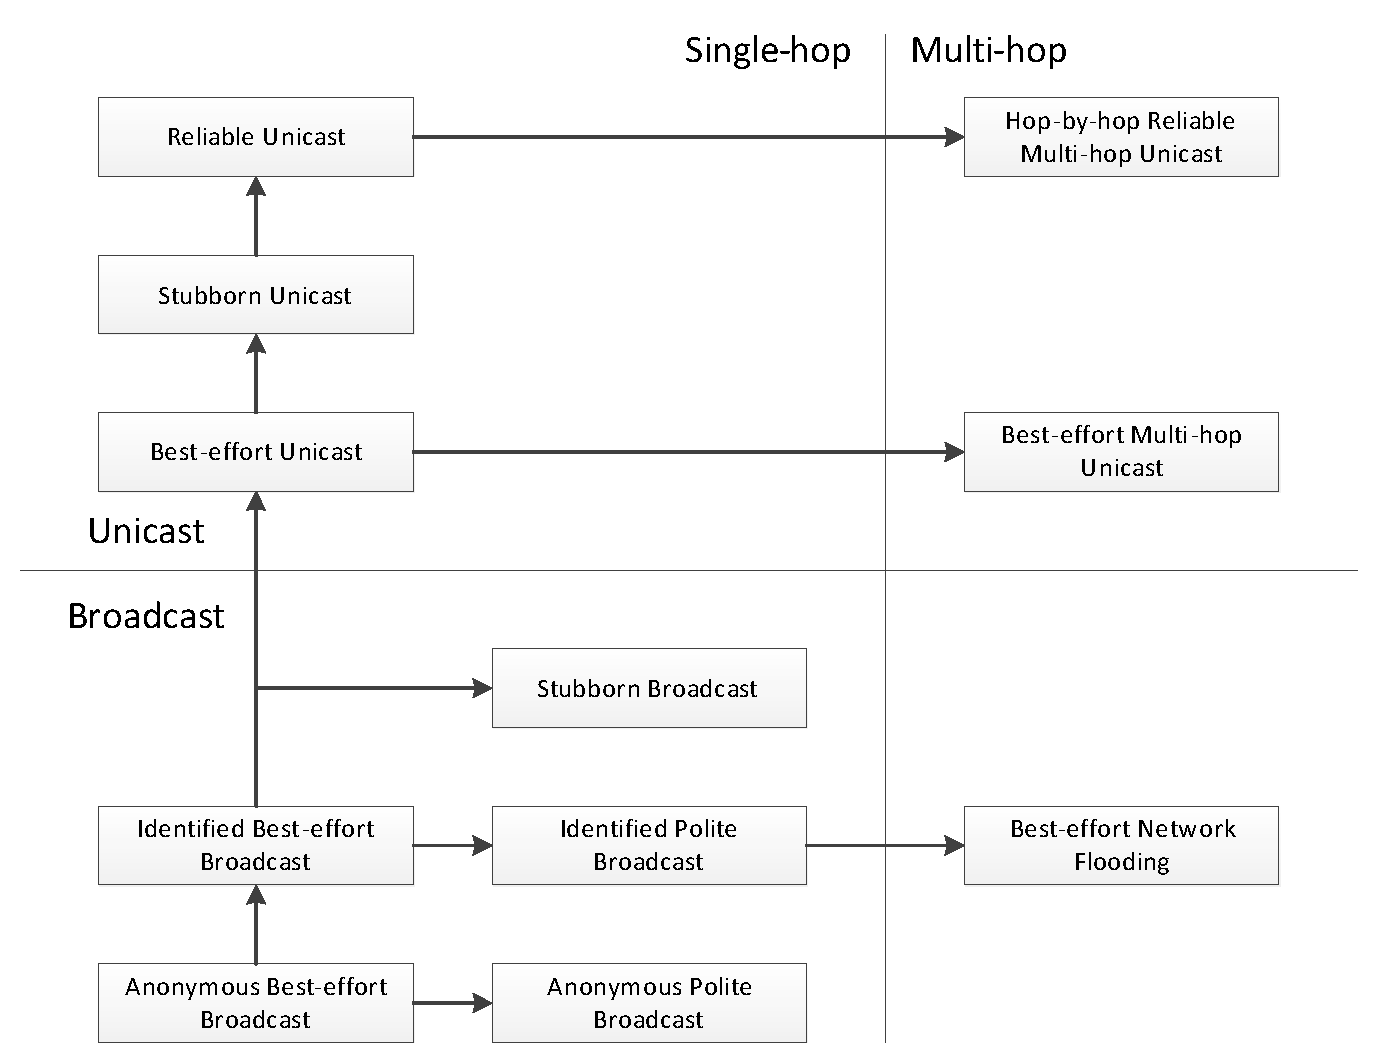
\includegraphics[width=\textwidth]{Diagrams/rime-stack}
	\caption{The communication primitives in the Rime network stack \cite{Dunkels:2007:ACA:1322263.1322295}}
\end{figure}

\begin{table}[H]
	\centering
	\begin{tabular}{ | l | l | l | }
		\hline
		Name & Header & Address \\
		\hline
		Anonymous Broadcast & abc.h & \url{contiki.sourceforge.net/docs/2.6/a01717.html} \\
		Broadcast & broadcast.h & \url{contiki.sourceforge.net/docs/2.6/a01720.html} \\
		Stubborn Broadcast & stbroadcast.h & \url{contiki.sourceforge.net/docs/2.6/a01739.html} \\
		Anonymous Polite Broadcast & polite.h & \url{contiki.sourceforge.net/docs/2.6/a01730.html} \\
		Polite Broadcast & ipolite.h & \url{contiki.sourceforge.net/docs/2.6/a01724.html} \\
		Unicast & unicast.h & \url{contiki.sourceforge.net/docs/2.6/a01738.html} \\
		Stubborn Unicast & stunicast.h & \url{contiki.sourceforge.net/docs/2.6/a01740.html} \\
		Reliable Unicast & runicast.h & \url{contiki.sourceforge.net/docs/2.6/a01738.html} \\
		Network Flooding & netflood.h & \url{contiki.sourceforge.net/docs/2.6/a01728.html} \\
		Multi-hop Unicast & multihop.h & \url{contiki.sourceforge.net/docs/2.6/a01726.html} \\
		Reliable Multi-hop Unicast & rmh.h & \url{contiki.sourceforge.net/docs/2.6/a01732.html} \\
		\hline
		\hline
		Mesh & mesh.h & \url{contiki.sourceforge.net/docs/2.6/a01725.html} \\
		Collect & collect.h & \url{contiki.sourceforge.net/docs/2.6/a01723.html} \\
		Trickle & trickle.h & \url{contiki.sourceforge.net/docs/2.6/a01742.html} \\
		\hline
	\end{tabular}
	\caption{Communication Primitives headers and documentation location}
\end{table}


\begin{table}[H]
	\centering
	\begin{tabular}{ | l | l | l | l | }
		\hline
		Name & Reliable & Target & Sender Known\\
		\hline
		Anonymous Broadcast & No & 1-hop neighbours & No\\
		Broadcast & No & 1-hop neighbours & Yes\\
		Stubborn Broadcast & No & 1-hop neighbours & No\\
		Anonymous Polite Broadcast & No & 1-hop neighbours & No\\
		Polite Broadcast & No & 1-hop neighbours & Yes\\
		Unicast & No & destination & Yes\\
		Stubborn Unicast & No & destination & Yes\\
		Reliable Unicast & Yes & destination & Yes\\
		Network Flooding & No & network & Yes\\
		Multi-hop Unicast & No & destination & Yes\\
		Reliable Multi-hop Unicast & Yes & destination & Yes\\
		\hline
		\hline
		Mesh & No & destination & Yes \\
		Collect & Yes & destination & Yes \\
		Trickle & Yes & network & No \\
		\hline
	\end{tabular}
	\caption{Communication Primitives behaviour}
\end{table}

\subsubsection{Anonymous Best-effort Broadcast}

This is the most basic kind of message transmission primitive in Contiki's Rime network stack. It broadcasts a single packet with a maximum length to its 1-hop neighbours. No information about the sender is included within the transmission. It is not usually the case that this type of broadcast is used, as more reliable, more informative primitives (that are built on this one) are often used instead.

\begin{listing}[H]
\begin{minted}[fontsize=\small]{c}
void abc_open(struct abc_conn *c, uint16_t channel, const struct abc_callbacks *u);
void abc_close(struct abc_conn *c);
int abc_send(struct abc_conn *c);

struct abc_callbacks {
   void(* recv)(struct abc_conn *ptr);
};
\end{minted}
\caption{Contiki Anonymous Best-effort Broadcast APIs}
\end{listing}

\subsubsection{Identified Best-effort Broadcast}

This broadcast primitive is essentially the same as the Anonymous Best-effort Broadcast primitive, except for the fact that the address of the sender is included within the header of the message. This address is then made available to the developer when the \verb|recv| callback is called (as can been seen in \autoref{lst:IBEB}).

\begin{listing}[H]
\begin{minted}[fontsize=\small]{c}
void broadcast_open(struct broadcast_conn *c, uint16_t channel,
                    const struct broadcast_callbacks *u);
void broadcast_close(struct broadcast_conn *c);
int broadcast_send(struct broadcast_conn *c);

struct broadcast_callbacks {
   void(* recv)(struct broadcast_conn *ptr, const rimeaddr_t *sender);
};
\end{minted}
\caption{Contiki Identified Best-effort Broadcast APIs}
\label{lst:IBEB}
\end{listing}


\subsubsection{Stubborn Broadcast}

\begin{listing}[H]
\begin{minted}[fontsize=\small]{c}
void stbroadcast_open(struct stbroadcast_conn *c, uint16_t channel,
                      const struct stbroadcast_callbacks *u);
void stbroadcast_close(struct stbroadcast_conn *c);
void stbroadcast_set_timer(struct stbroadcast_conn *c, clock_time_t t);
int stbroadcast_send_stubborn(struct stbroadcast_conn *c, clock_time_t t);
void stbroadcast_cancel(struct stbroadcast_conn *c);

struct stbroadcast_callbacks {
   void (* recv)(struct stbroadcast_conn *c);
   void (* sent)(struct stbroadcast_conn *c);
};
\end{minted}
\caption{Contiki Stubborn Broadcast APIs}
\end{listing}

\subsubsection{Anonymous Polite Broadcast}

\begin{listing}[H]
\begin{minted}[fontsize=\small]{c}
void polite_open(struct polite_conn *c, uint16_t channel,
                 const struct polite_callbacks *cb);
void polite_close(struct polite_conn *c);
int polite_send(struct polite_conn *c, clock_time_t interval, uint8_t hdrsize);
void polite_cancel(struct polite_conn *c);

struct stbroadcast_callbacks {
   void(* recv)(struct polite_conn *c);
   void(* sent)(struct polite_conn *c);
   void(* dropped)(struct polite_conn *c);
};
\end{minted}
\caption{Contiki Anonymous Polite Broadcast APIs}
\end{listing}

\subsubsection{Identified Polite Broadcast}

\begin{listing}[H]
\begin{minted}[fontsize=\small]{c}
void ipolite_open(struct ipolite_conn *c, uint16_t channel,
                  uint8_t maxdups, const struct ipolite_callbacks *cb);
void ipolite_close(struct ipolite_conn *c);
int ipolite_send(struct ipolite_conn *c, clock_time_t interval, uint8_t hdrsize);
void ipolite_cancel(struct ipolite_conn *c);

struct stbroadcast_callbacks {
   void(* recv)(struct ipolite_conn *c, const rimeaddr_t *from)
   void(* sent)(struct ipolite_conn *c);
   void(* dropped)(struct ipolite_conn *c);
};
\end{minted}
\caption{Contiki Identified Polite Broadcast APIs}
\end{listing}

\subsubsection{Best-effort Unicast}

\begin{listing}[H]
\begin{minted}[fontsize=\small]{c}
void unicast_open(struct unicast_conn *c, uint16_t channel, const struct unicast_callbacks *u);
void unicast_close(struct unicast_conn *c);
int unicast_send(struct unicast_conn *c, const rimeaddr_t *receiver);

struct unicast_callbacks {
   void (* recv)(struct unicast_conn *c, const rimeaddr_t *from);
   void (* sent)(struct unicast_conn *ptr, int status, int num_tx);
};
\end{minted}
\caption{Contiki Best-effort Unicast APIs}
\end{listing}

\subsubsection{Stubborn Unicast}

\begin{listing}[H]
\begin{minted}[fontsize=\small]{c}
void stunicast_open(struct stunicast_conn *c, uint16_t channel,
                    const struct stunicast_callbacks *u);
void stunicast_close(struct stunicast_conn *c);
int stunicast_send_stubborn(struct stunicast_conn *c,
                            const rimeaddr_t *receiver, clock_time_t rxmittime);
void stunicast_cancel(struct stunicast_conn *c);
int stunicast_send(struct stunicast_conn *c, const rimeaddr_t *receiver);
void stunicast_set_timer(struct stunicast_conn *c, clock_time_t t);
rimeaddr_t *stunicast_receiver(struct stunicast_conn *c);

struct stunicast_callbacks {
   void (* recv)(struct stunicast_conn *c, const rimeaddr_t *from);
   void (* sent)(struct stunicast_conn *c, int status, int num_tx);
};
\end{minted}
\caption{Contiki Stubborn Unicast APIs}
\end{listing}

This is in fact anonymous, it will not send the address of the node that send the message in the header of the message. If a node needs to know who sent the message, then the sender's address should be included in the body.


\subsubsection{Reliable Unicast}

\begin{listing}[H]
\begin{minted}[fontsize=\small]{c}
void runicast_open(struct runicast_conn *c, uint16_t channel,
                   const struct runicast_callbacks *u);
int runicast_send(struct runicast_conn *c, const rimeaddr_t *receiver,
                  uint8_t max_retransmissions);
uint8_t runicast_is_transmitting(struct runicast_conn *c);

struct runicast_callbacks {
   void (* recv)(struct runicast_conn *c, const rimeaddr_t *from, uint8_t seqno);\cite{
   void (* sent)(struct runicast_conn *c, const rimeaddr_t *to, uint8_t retransmissions);
   void (* timedout)(struct runicast_conn *c, const rimeaddr_t *to, uint8_t retransmissions);
};
\end{minted}
\caption{Contiki Reliable Unicast APIs}
\end{listing}

\subsubsection{Best-effort Network Flooding}

\begin{listing}[H]
\begin{minted}[fontsize=\small]{c}
void netflood_open(struct netflood_conn *c, clock_time_t queue_time,
                   uint16_t channel, const struct netflood_callbacks *u);
void netflood_close(struct netflood_conn *c);
int netflood_send(struct netflood_conn *c, uint8_t seqno);

struct netflood_callbacks {
   int (* recv)(struct netflood_conn *c, const rimeaddr_t *from,
                const rimeaddr_t *originator, uint8_t seqno, uint8_t hops);
   void (* sent)(struct netflood_conn *c);
   void (* dropped)(struct netflood_conn *c);
};
\end{minted}
\caption{Contiki Best-effort Network Flooding APIs}
\end{listing}

\subsubsection{Best-effort Multi-hop Unicast}

\begin{listing}[H]
\begin{minted}[fontsize=\small]{c}
void rmh_open(struct rmh_conn *c, uint16_t channel, const struct rmh_callbacks *u);
void rmh_close(struct rmh_conn *c);
int rmh_send(struct rmh_conn *c, rimeaddr_t *to, uint8_t num_rexmit, uint8_t max_hops);

struct rmh_callbacks {
   void (* recv)(struct rmh_conn *ptr, rimeaddr_t *sender, uint8_t hops);
   rimeaddr_t *(* forward)(struct rmh_conn *ptr,
                          const rimeaddr_t *originator,
                          const rimeaddr_t *dest,
                          const rimeaddr_t *prevhop,
                          uint8_t hops);
};
\end{minted}
\caption{Contiki Best-effort Multi-hop Unicast APIs}
\end{listing}

\subsubsection{Hop-by-hop Reliable Multi-hop Unicast}

\begin{listing}[H]
\begin{minted}[fontsize=\small]{c}
void multihop_open(struct multihop_conn *c, uint16_t channel,
                   const struct multihop_callbacks *u);
void multihop_close(struct multihop_conn *c);
int multihop_send(struct multihop_conn *c, const rimeaddr_t *to);
void multihop_resend(struct multihop_conn *c, const rimeaddr_t *nexthop);

struct multihop_callbacks {
   void (* recv)(struct multihop_conn *ptr,
                 const rimeaddr_t *sender,
                 const rimeaddr_t *prevhop,
                 uint8_t hops);
   rimeaddr_t *(* forward)(struct multihop_conn *ptr,
                           const rimeaddr_t *originator,
                           const rimeaddr_t *dest,
                           const rimeaddr_t *prevhop,
                           uint8_t hops);
};
\end{minted}
\caption{Contiki Hop-by-hop Reliable Multi-hop Unicast APIs}
\end{listing}


\subsection{Mesh Network Protocol}

\begin{listing}[H]
\begin{minted}[fontsize=\small]{c}
void mesh_open(struct mesh_conn *c, uint16_t channels, const struct mesh_callbacks *callbacks);
void mesh_close(struct mesh_conn *c);
int mesh_send(struct mesh_conn *c, const rimeaddr_t *dest);

struct mesh_callbacks {
   /** Called when a packet is received. */
   void (* recv)(struct mesh_conn *c, const rimeaddr_t *from, uint8_t hops);
   /** Called when a packet, sent with mesh_send(), is actually transmitted. */
   void (* sent)(struct mesh_conn *c);
   /** Called when a packet, sent with mesh_send(), times out and is dropped. */
   void (* timedout)(struct mesh_conn *c);
};
\end{minted}
\caption{Contiki Mesh Network APIs}
\end{listing}


\subsection{Collect Network Protocol}

\begin{listing}[H]
\begin{minted}[fontsize=\small]{c}
void collect_open(struct collect_conn *c,
                  uint16_t channels, uint8_t is_router,
                  const struct collect_callbacks *callbacks);
void collect_close(struct collect_conn *c);
int collect_send(struct collect_conn *c, int rexmits);
void collect_set_sink(struct collect_conn *c, int should_be_sink);
int collect_depth(struct collect_conn *c);
const rimeaddr_t *collect_parent(struct collect_conn *c);
void collect_set_keepalive(struct collect_conn *c, clock_time_t period);

struct collect_callbacks {
   void (* recv)(const rimeaddr_t *originator, uint8_t seqno,
                 uint8_t hops);
};
\end{minted}
\caption{Contiki Collect Network APIs}
\end{listing}


\subsection{Trickle Network Protocol}

\begin{listing}[H]
\begin{minted}[fontsize=\small]{c}
void trickle_open(struct trickle_conn *c, clock_time_t interval,
                  uint16_t channel,
                  const struct trickle_callbacks *cb);
void trickle_close(struct trickle_conn *c);
void trickle_send(struct trickle_conn *c);

struct trickle_callbacks {
   void (* recv)(struct trickle_conn *c);
};
\end{minted}
\caption{Contiki Trickle Network APIs}
\end{listing}


\subsection{Network Channels}

Channels in Contiki are virtual \cite{tel-aviv-contiki-exercises, Dunkels:2007:ACA:1322263.1322295}. This means that when a connection is opened if you do not want to receive packets from another connection then a different channel should be used. It does not mean that different radio frequencies are used. To use different radio frequencies the function \verb|cc2420_set_channel| should be used to change the frequency messages are broadcasted on.


\subsection{Timers}

\subsubsection{Event Timer}

\url{http://contiki.sourceforge.net/docs/2.6/a01667.html}

\subsubsection{Callback Timer}

\url{http://contiki.sourceforge.net/docs/2.6/a01666.html}


\subsection{Optimisation}

\subsection{LTO and Whole Program}

Its is a shame that the developers of Contiki seem unwilling to support LTO (Link-Time Optimisations) that could greatly decrease the size of the binary and optimise the code \url{http://comments.gmane.org/gmane.comp.hardware.texas-instruments.msp430.gcc.user/11006}.

\subsection{Memory}



\clearpage

% !TeX root = Report.tex
\section{Implemented Algorithms}

\dirtree{%
.1 Common/.
.2 containers/.
.3 linked-list.[h/c].
.3 array-list.[h/c].
.3 unique-array.[h/c].
.3 map.[h/c].
.2 net/.
.3 eventupdate.[h/c].
.3 multipacket.[h/c].
.3 nhopflood.[h/c].
.3 nhopreq.[h/c].
.3 rimeaddr-helpers.[h/c].
.3 tree-aggregator.[h/c].
.2 debug-helper.[h/c].
.2 led-helper.[h/c].
.2 random-range.[h/c].
.2 sensor-converter.[h/c].
}

\subsection{Container Library}

Contiki comes with a list container \footnote{Header: \url{https://github.com/contiki-os/contiki/blob/master/core/lib/list.h} Source: \url{https://github.com/contiki-os/contiki/blob/master/core/lib/list.c}}, however, when we were developing with their linked list we found that it was awkward to use in some situations (for instance creating an array of lists) so we decided that we needed to find a better list library. Our problem was that other container libraries were unlikely to be optimised to the low memory requirements or support the special compile chain used by Contiki. So rather than waste time searching and integrating an external library we decided to write our own set of containers. By doing the main benefit we gained was that we knew how the containers worked so had a better understanding how to use them.

Another reason to develop our own containers was that we desired an list where the data was stored in an array, this was for because it provides lower memory overhead and the types of operations we would be performing (append and empty) meant that an array backed list would be better. The lower memory overhead comes from the fact that an array-based list doesn't need to store a pointer to the next element as it is implicit (due to the contiguous memory) that a pointer to the current element's pointer plus one is the next element. This means that in a list of $N$ items our singly linked list implementation will require $(\text{sizeof}(T) + \text{sizeof}(void *) \times 2) \times N$ bytes of memory, whereas our array list implementation will require $(\text{sizeof}(T) + \text{sizeof}(void *)) \times N$ bytes of memory.

Our linked list implementation uses more memory compared to Contiki's implementation because their list is \emph{intrusive}\footnote{Boost Containers: \url{http://www.boost.org/doc/libs/1\_53\_0/doc/html/intrusive/presenting\_containers.html}}. What is meant by this is that the pointer to the next item in the list is contained in the structure stored in the list \cite{?}. Meaning their list uses the same amount of memory as our array list. However, because the list is intrusive it makes it more difficult to use as the implementation detail leaks into the structure using the library, this was why developing our own non-intrusive list made it easier to develop code.

We also developed containers that helped abstract certain concepts (such as list uniqueness or accessing elements by key) to decrease code duplication and allow us to express the code in a higher-level way making implementation easier. One thing to note is that for the containers we did not focus on implementing some of their functions to the standard complexity. For example our map implementation has requires O(N) for both insert and fetching, where these may be implemented as O(1) on average (hash tables) or O(log N) (trees), however due to the requirements of low memory we decided to keep using the array as the backing store for the data with the aim to keep memory for at the expense of non-optimal container management functions. The increased time complexity should make little difference as the containers tend to have few elements in them (i.e. hundreds rather than millions, where complexity would start to be important \cite{?}).

Finally, all of these custom containers are tested by a test suite that checks for functional correctness. Also the test suite was run using \verb|valgrind|\footnote{\url{http://valgrind.org/info/tools.html}} to check for memory leaks and corruption.


\subsection{Network Library}

\subsubsection{Event Update}

\begin{figure}[H]
  \centering
  \begin{boxedminipage}{\linewidth}
    % 
    \null Process $j$ - \res{event-update}\\
    %
    \null \textbf{variables}\\
    %
    \null\qq \var{period}: timer init $P_{generate}$;\\~\\
    %
    \null\qq \% The previous node data sent to the network\\
    \null\qq \var{previous}: struct init $\bot$;\\~\\
    %
    \null \textbf{constants}\\
    %
    \null\qq \% Generate Period, how often we should check for a change in the data\\
    \null\qq \var{$P_{generate}$}: time;\\~\\
    %
    \null\qq \% Checks if the data differs\\
    \null\qq \var{differs}: function takes (struct, struct) returns boolean;\\~\\
    %
    \null\qq \% Gets the data of the current node\\
    \null\qq \var{data}: function takes () returns struct;\\~\\
    %
    \null\qq \% The probability of sending our data, even if no change occurred\\
    \null\qq \var{chance}: real;\\~\\
    %
    \null \textbf{parameters}\\
    %
    \null\qq \% The distance we need to send information\\
    \null\qq \var{distance}: int;\\~\\
    %
    \null \textbf{actions}\\
    %
    %
    \null\qq \% Check for changes\\
    \null\qq \emph{check}::~\res{timeout}(\var{period}) $\rightarrow$\\
    \null\qq\qq $\var{force} \assign \res{RandReal}(0, 1) \leq \var{chance}$;\\
    \null\qq\qq $\var{changed} \assign \var{previous} = \bot \lor \var{differs}(\var{data}(), \var{previous})$;\\
    \null\qq\qq \res{if} ($\var{force} \lor \var{changed}$) \res{then}\\
    \null\qq\qq\qq $\var{previous} \assign \var{data}()$;\\
    \null\qq\qq\qq \res{nhopflood}$\langle j, \var{previous}, \var{distance}\rangle$;\\
    \null\qq\qq \res{fi}; \\
    \null\qq\qq \res{set}($\mathit{period}$, $P_{generate}$); \\~\\
    %
    %
    \null\qq \% Receiving Change message\\
    \null\qq \emph{receive}::~\res{nhopflood.recv}$\langle source, data, hops\rangle \rightarrow$\\
    \null\qq\qq \% Prevent delivery if being told that the current node's data has changed\\
    \null\qq\qq \res{if} ($j \not= source$) \res{then} \\
    \null\qq\qq\qq \% Inform library caller of data change\\
    \null\qq\qq\qq \res{data-changed-callback}(\var{data}, \var{hops}); \\
    \null\qq\qq \res{fi}; \\
    %
    %
  \end{boxedminipage}
  \caption{Event Update Broadcast Algorithm}
\end{figure}


\subsubsection{Multi-Packet}

In Contiki sending a single packet has its limits, there is only so much data you can get in a single packet. There are two C macros that are relevant to this \verb|PACKETBUF_HDR_SIZE| which is set to 48 bytes and \verb|PACKETBUF_SIZE| which is set to 128 bytes\footnote{packetbuf.h \url{http://contiki.sourceforge.net/docs/2.6/a00302.html}}. This means that in general we will only be able to send a packet containing 128 bytes of information, but what if we have a data structure that spans 300 bytes? Then we will need to have a way to send multiple packets and a receiver that can put the packets back together in the correct way to deliver the data.

Contiki's data transfer primitives for their RIME protocols are fairly hidden because of their focus on uIPv6. We found \verb|ruldolph0| first \footnote{ruldolph0 \url{http://contiki.sourceforge.net/docs/2.6/a01735.html}} and then \verb|rucb| (Reliable Unicast Bulk Transfer) much later \footnote{rucb \url{http://contiki.sourceforge.net/docs/2.6/a00365.html}}. However, both of them have problems, the API is very convoluted and seems more geared towards sending very large files across the network. This is very different to our aim, which is to send relatively small packets of data to a specific neighbour. So we wrote our own API that would split data of any given size and reassemble it once received, our API was not focused on processing data chunks like \verb|ruldolph0| or \verb|rucb|, but simply operated on a block of memory given to it. This is a case where a simpler API made development much easier for us. Admittedly because our implementation uses dynamic memory allocation it could potentially perform worse, but because the energy of sending and receiving messages dwarfs the energy usage of the CPU, we feel that easier development tradeoff it worth it. Also, now that code has been written to use this API, the \verb|multipacket| library itself could always be rewritten to use \verb|rucb| as a base to run more efficiently.


\subsubsection{N-Hop Flood}

\subsubsection{N-Hop Request}
Contiki provides broadcast primitives to allow the flooding of messages through the network, however the \verb|trickle|\cite{Levis04trickle} primitive only allows a single source node\footnote{trickle.h \url{http://contiki.sourceforge.net/docs/2.6/a00381.html}}, which presents a problem, when multiple nodes are attempting to send a message N-hops away. 
In some cases \verb|reliable unicast| could be used to target the specific nodes for which the message is intended. This, however, is not suitable when the identifies of the nodes is not known, or in situations when storing routing tables is not appropriate. 

Our response to this was to develop a primitive which would flood the network, a fixed number of hops from the source, whilst allowing multiple nodes to use the same primitive, with different messages. Our implementation uses a \verb|stubborn broadcast| to pass the message along a chain, only rebroadcasting the message when the hop limit (the number of hops the message is intended to travel) has not been reached. If a message has been seen before by a node (and the number of hops left is lower than before) it is simply ignored and not passed on. In the case where the hop count for a 
duplicate message is higher than the previously seen count, it is then rebroadcast, so that all the intended recipients will receive the message.  
After a fixed time, messages are then sent back to the source along a chain, this time is reset whenever a message with a higher hop count is seen.  Each node stores the ID of the node that it received the message from, and the response message is sent back to that node. In turn, that node will forward the message to the node it received the original message from, eventually the message will end up at the source, to be processed.

%TODO: Note about performance maybe?
%Could also put a graphic of the chain here too

\begin{figure}[H]
  \centering
  \begin{boxedminipage}{\linewidth}
    % 
    \null Process $j$ - \verb|n-hop-req|\\
    %
    \null \textbf{parameters}\\
    %
    \null\qq \% The number of hops left to send a message\\
    \null\qq \var{hop\_limit}: int\\~\\
    %
    %
    \null \textbf{variables}\\
    %
    \null\qq \%The nodes a given message was seen from\\
    \null\qq \var{mote\_records}: map\\~\\
    %
    %
    \null \textbf{constants}\\
    %
    \null\qq \% Send Data Period, the time between receiving a request for data, and sending it\\
    \null\qq \var{$P_{send\_data}$}: time;\\~\\
    %
    %
    \null \textbf{actions}\\
    %
    %
    \null\qq \% Receiving Message\\
    \null\qq \emph{receive}::~\res{recv}$\langle source, data, hop\_count, id\rangle \rightarrow$\\
    \null\qq\qq \res{if} ($mote\_records.contains(id)$) \res{then}\\
    \null\qq\qq\qq \res{if} ($mote\_records.hop\_count(id) < hop\_count$) \res{then} \\
    \null\qq\qq\qq\qq \res{stbroadcast.send($message$,$hop\_count -1$)};\\
    \null\qq\qq\qq\qq \res{$mote\_records$.replace($id$,$hop\_count$)};\\
    \null\qq\qq\qq\qq \res{\var{$P_{send\_data}$}.restart()}\\
    \null\qq\qq\qq \res{fi;}\\
    \null\qq\qq \res{else}\\
    \null\qq\qq\qq \res{stbroadcast.send($message$,$hop\_count -1$)};\\
    \null\qq\qq\qq \res{$mote\_records$.add($id$,$data$,$source$,$hop\_count$)};\\
    \null\qq\qq\qq \res{\var{$P_{send\_data}$}.start()}\\
    \null\qq\qq \res{fi;}\\~\\
    %
    %
    \null\qq \% Sending Data\\
    \null\qq \emph{send\_data}:~\res{timeout}(\var{$P_{send\_data}$})$\rightarrow$\\
    \null\qq\qq \res{runicast.send}($j$,$mote\_records.getMote(id)$, $data$);\\~\\
    %
    %
    \null\qq \% Recieved Data\\
    \null\qq \emph{recv\_data}:~\res{runicast.recv}$\langle source, data, id\rangle \rightarrow$\\
    \null\qq\qq \res{if} ($mote\_records.getMote(id)$ == $self$) \res{then}\\
    \null\qq\qq\qq \% Process Data\\
    \null\qq\qq \res{else}\\
    \null\qq\qq\qq \res{runicast.send}($mote\_records.getMote(id)$, $data$);\\
    \null\qq\qq \res{fi;}\\
    %
    %
  \end{boxedminipage}
  \caption{N-Hop Request Algorithm}
  \label{fig:n-hop-req-algorithm}
\end{figure}

\subsubsection{Tree Aggregation}

As has been previously mentioned Tree Aggregation is a very useful technique employed in wireless sensor networks to aggregate a set of data to a single node in the network. It is very useful because of its ability to convey the same amount of data in potentially fewer messages. The algorithm works by first creating a tree structure such that nodes know of a parent node that they should unicast their messages to. Once this tree is set up the nodes (typically leaf nodes) unicast data to their parents, this can either happen when an event occurs or it can happen periodically. When a parent node receives a message it waits for a certain amount of time for more messages to arrive, every message it receives is stored and aggregated. After the time period is up the aggregated data is forwarded to its parent node. Once the data reaches the destination it is delivered to the user of the library.


The user of this library needs to implement four important functions:
\begin{enumerate}
\item[$\otimes_{agg}$] This function aggregates stored data with data message that has been received
\item[$\otimes_{own}$] This function aggregates the node's own data into the stored data
\item[$\otimes_{read}$] This function does the initial reading of data from a message and creates the local stored data
\item[$\otimes_{write}$] This function writes the local stored data back to a packet
\end{enumerate}


\begin{figure}[H]
  \centering
  \begin{boxedminipage}{\linewidth}
    % 
    \null Process $j$ - \res{tree-aggregation}\\
    %
    \null \textbf{variables}\\
    %
    \null\qq \var{parentdetect}: timer init $\bot$;\\~\\
    %
    \null\qq \var{seensetup}, \var{collecting}, \var{leaf}: bool init $False$, $False$, $True$;\\~\\
    %
    \null\qq \var{besthop}: int init $INTMAX$;\\~\\
    %
    \null\qq \var{bestparent}: address init $\bot$;\\~\\~\\
    %
    \null\qq \var{aggregation}: timer init $\bot$;\\~\\
    %
    \null\qq \var{collecting}: bool init $False$;\\~\\
    %
    \null\qq \var{stored}: struct init $\bot$;\\~\\
    %
    \null \textbf{constants}\\
    %
    \null\qq \% How long to wait for messages to aggregate before forwarding what the node has\\
    \null\qq \var{$P_{aggregation}$}: time;\\~\\
    %
    \null\qq \% How long to wait for parents to be detected\\
    \null\qq \var{$P_{parentdetect}$}: time;\\~\\
    %
    \null \textbf{parameters}\\
    %
    \null\qq \% The address of the node data should be aggregated to\\
    \null\qq \var{sink}: address;\\
    %
  \end{boxedminipage}
  \caption{Tree Aggregation Algorithm - variables}
\end{figure}

\begin{figure}[H]
  \centering
  \begin{boxedminipage}{\linewidth}
    \null \textbf{actions}\\
    %
    %
    \null\qq \% Set up tree: initialise\\
    \null\qq \emph{starup}::~\res{init} $\rightarrow$\\
    \null\qq\qq \res{bcast}$\langle j, \bot, 1\rangle$;\\~\\
    %
    %
    \null\qq \% Set up tree: receive message\\
    \null\qq \emph{receive}::~\res{recv}$\langle source, parent, hops\rangle \rightarrow$\\
    \null\qq\qq \res{if} ($j \not= sink$) \res{then} \\
    \null\qq\qq\qq \res{if} ($\lnot\var{seensetup}$) \res{then} \\
    \null\qq\qq\qq\qq $\var{seensetup} \assign True$; \\
    \null\qq\qq\qq\qq \res{set}($\mathit{parentdetect}$, $P_{parentdetect}$); \\
    \null\qq\qq\qq \res{fi}; \\
    \null\qq\qq\qq \res{if} ($\var{hops} < \var{besthop}$) \res{then} \\
    \null\qq\qq\qq\qq $\var{bestparent}, \var{besthop} \assign \var{source}, \var{hops}$; \\
    \null\qq\qq\qq \res{fi}; \\
    \null\qq\qq\qq \res{if} ($\var{leaf} \land \var{j} = \var{parent}$) \res{then} \\
    \null\qq\qq\qq\qq $\var{leaf} \assign False$; \\
    \null\qq\qq\qq \res{fi}; \\
    \null\qq\qq \res{fi}; \\~\\
    %
    %
    \null\qq \% Set up tree: finish detecting parents\\
    \null\qq \emph{check}::~\res{timeout}(\var{parentdetect}) $\rightarrow$\\
    \null\qq\qq \res{if} ($\var{besthop} = INTMAX$) \res{then} \\
    \null\qq\qq\qq \res{bcast}$\langle j, \var{bestparent}, INTMAX\rangle$;\\
    \null\qq\qq \res{else} \\
    \null\qq\qq\qq \res{bcast}$\langle j, \var{bestparent}, \var{besthop} + 1\rangle$;\\
    \null\qq\qq \res{fi}; \\
    %
    %
  \end{boxedminipage}
  \caption{Tree Aggregation Algorithm - Setting up tree}
\end{figure}


\begin{figure}[H]
  \centering
  \begin{boxedminipage}{\linewidth}
    \null \textbf{actions}\\
    %
    %
    \null\qq \% Send data function\\
    \null\qq \emph{send}::~\res{function}$\langle data\rangle \rightarrow$\\
    \null\qq\qq \res{multipacket.unicast}$\langle \var{bestparent}, data\rangle$;\\~\\
    %
    %
    \null\qq \% Set up tree: receive message\\
    \null\qq \emph{receive}::~\res{multipacket.recv}$\langle source, data\rangle \rightarrow$\\
    \null\qq\qq \res{if} ($j = sink$) \res{then} \\
    \null\qq\qq\qq $\var{stored} \assign \otimes_{read}(data)$; \\
    \null\qq\qq\qq $\var{stored} \assign \otimes_{own}(\var{stored})$; \\
    \null\qq\qq\qq $\res{deliver}(\otimes_{write}(\var{stored}))$; \\
    \null\qq\qq \res{else} \\
    \null\qq\qq\qq \res{if} ($\var{collecting}$) \res{then} \\
    \null\qq\qq\qq\qq $\var{stored} \assign \otimes_{agg}(\var{stored}, \var{data})$; \\
    \null\qq\qq\qq \res{else} \\
    \null\qq\qq\qq\qq $\var{stored} \assign \otimes_{read}(data)$; \\
    \null\qq\qq\qq\qq $\var{collecting} \assign True$; \\
    \null\qq\qq\qq\qq \res{set}($\mathit{aggregation}$, $P_{aggregation}$); \\
    \null\qq\qq\qq \res{fi}; \\
    \null\qq\qq \res{fi}; \\~\\
    %
    %
    \null\qq \% Set up tree: finish detecting parents\\
    \null\qq \emph{finishagg}::~\res{timeout}(\var{aggregation}) $\rightarrow$\\
    \null\qq\qq \res{multipacket.unicast}$\langle \var{bestparent}, \otimes_{write}(\var{stored})\rangle$;\\
    \null\qq\qq $\var{collecting} \assign False$; \\
    \null\qq\qq $\var{stored} \assign \bot$; \\
    %
    %
  \end{boxedminipage}
  \caption{Tree Aggregation Algorithm - Sending data}
\end{figure}


\begin{figure}[ht!]
\centering
\subfigure[Example Network]{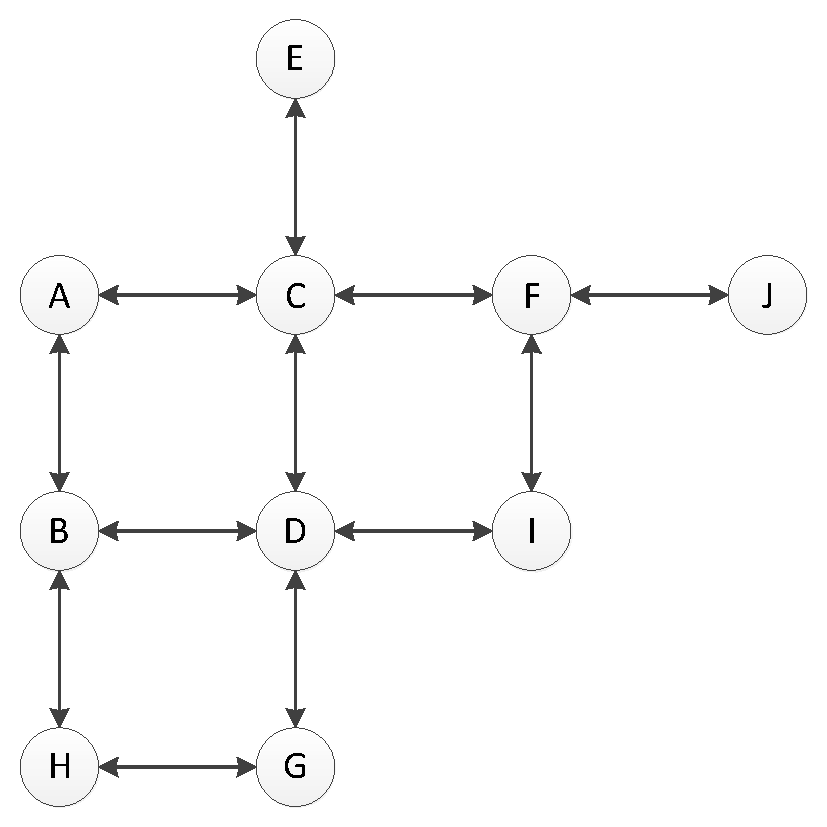
\includegraphics[width=0.5\textwidth]{Diagrams/neighbour-network}}

\subfigure[Logical Tree imposed on network]{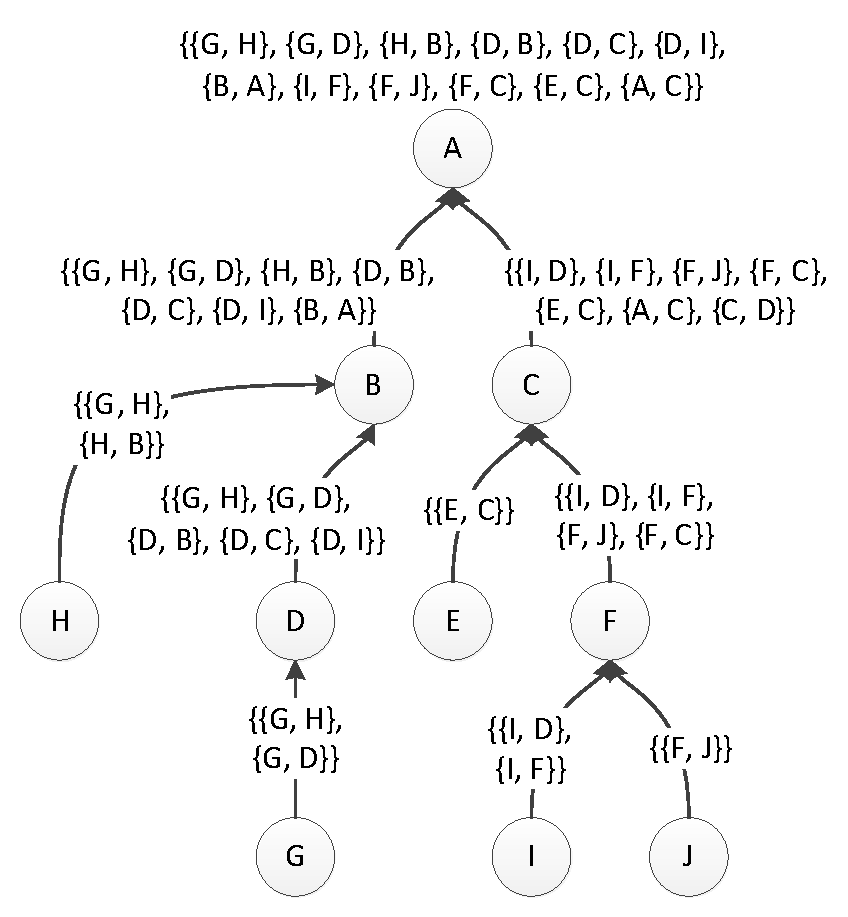
\includegraphics[width=0.5\textwidth]{Diagrams/neighbour-tree-structure}}
\end{figure}

\subsubsection{Neighbour Detect}

To aid in debugging a vital piece of information that will be required about the network is its topology. Trying to analyse network state without knowing which nodes are neighbours of other nodes, makes drawing meaningful conclusions from that data much harder. This meant that we needed a way to send neighbour information back to the sink. Thankfully part of the job is already accomplished as Contiki comes with a library to perform neighbour detection\cite{?}. We extended that library in two ways.

The first was to add more features to Contiki's neighbour detect library. As that library was very simple and supported only saying that a neighbour had been detected (with the option of providing a integer value as well). As we were aiming for this code to support changes in the network, such as nodes leaving or joining neighbourhoods, we added the concept of a round. Instead of just knowing about neighbours at that instant in time, it allowed the library to maintain some kind of history about what nodes were neighbours of other nodes in the past. Whenever new nodes are detected they are recorded, however, if a node has not been detected for a certain number of rounds then that node is removed from the record.

\begin{figure}[ht!]
\centering
\subfigure[Node A requesting neighbour data]{\includegraphics[width=0.25\textwidth]{Diagrams/neighbour-request}}
\subfigure[Node A receiving neighbour data]{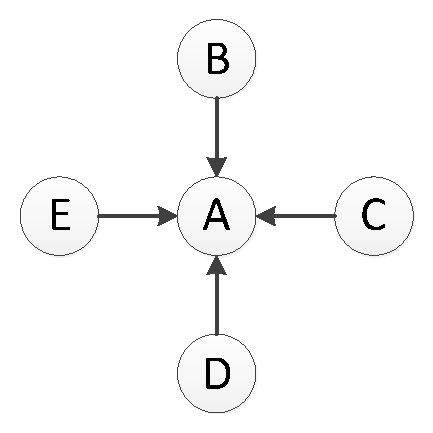
\includegraphics[width=0.25\textwidth]{Diagrams/neighbour-report}}
\caption{Nodes asking for and receiving neighbour data}
\end{figure}

\begin{figure}[H]
  \centering
  \begin{boxedminipage}{\linewidth}
    % 
    \null Process $j$ - \res{neighbourdetect}\\
    %
    \null \textbf{variables}\\
    %
    \null\qq \var{period}: timer init $P_{round}$;\\~\\
    %
    \null\qq \% The history of node\\
    \null\qq \var{previous}: map of address to int init $\emptyset$;\\~\\
    %
    \null\qq \% The current round\\
    \null\qq \var{count}: int init 0;\\~\\
    %
    \null \textbf{constants}\\
    %
    \null\qq \% Round Period\\
    \null\qq \var{$P_{round}$}: time;\\~\\
    %
    \null\qq \% The missed round threshold\\
    \null\qq \var{missed}: int;\\~\\
    %
    \null \textbf{actions}\\
    %
    %
    \null\qq \% Check for changes\\
    \null\qq \emph{round}::~\res{timeout}(\var{period}) $\rightarrow$\\
    \null\qq\qq $\var{previous} \assign \{ (addr, round) \in \var{previous} | count - round \geq missed \}$;\\
    \null\qq\qq \% Tell library caller that a round is finished\\
    \null\qq\qq \res{round-complete}(\res{values}(previous), \var{count});\\
    \null\qq\qq $\var{count} \assign \var{count} + 1$; \\
    \null\qq\qq \res{set}($\mathit{period}$, $P_{round}$); \\~\\
    %
    %
    \null\qq \% Receiving Neighbour Discovery message\\
    \null\qq \emph{neighbour}::~\res{neighbour\_discovery.recv}$\langle source, round\rangle \rightarrow$\\
    \null\qq\qq \% Update the round we last saw this node\\
    \null\qq\qq \res{if} ($source \in \res{keys}(\var{previous})$) \res{then} \\
    \null\qq\qq\qq \res{if} ($round > \var{previous}[\var{source}]$) \res{then} \\
    \null\qq\qq\qq\qq $\var{previous}[\var{source}] \assign \var{round}$; \\
    \null\qq\qq\qq \res{fi}; \\
    \null\qq\qq \res{else} \\
    \null\qq\qq\qq $\var{previous}[\var{source}] \assign \var{round}$; \\
    \null\qq\qq \res{fi}; \\~\\
    %
    %
  \end{boxedminipage}
  \caption{Neighbour Detect Algorithm}
  \label{algo:neighbour-detect}
\end{figure}

For this to be useful we needed a way to get this data back to the sink node. There are many ways to do this, but one of the best is aggregating along a tree because it can combine many messages into a single one and forward that aggregated message instead of lots of smaller messages \cite{?}. The Neighbour Aggregation part uses the Tree Aggregation library that we have developed, the function that is used to aggregate data together is $\cup$ (union), this allows data to be aggregated with other data and allows that data to be updated. The nodes own data is set to be $\res{node-data}$, where $\var{j}$ is the current node's address and $\res{round-data}$ is the set of node addresses provided by the $\res{round-complete}$ callback in \autoref{algo:neighbour-detect}.

\begin{equation}
\res{node-data} = \{\{\var{other}, \var{j}\} | \var{other} \in \res{round-data} \}
\end{equation}


\subsection{Clustering}

\begin{figure}[H]
  \centering
  \begin{boxedminipage}{\linewidth}
    % 
    \null Process $j$ - \res{clustering}\\
    %
    \null \textbf{variables}\\
    %
    \null\qq \% Boolean set to true when a node is elected to be a clusterhead\\
    %
    \null\qq \var{is\_CH}: bool init $False$;\\~\\
    %
    \null\qq \% Bool set to true on receipt of first setup message\\
    %
    \null\qq \var{seen\_setup}: bool init $False$;\\~\\
    %
    \null\qq \% Hop distance to best clusterhead\\
    %
    \null\qq \var{best\_hop}: int;\\~\\
    %
    \null\qq \% Address of best clusterhead\\
    %
    \null\qq \var{our\_CH}: address;\\~\\
    %
    \null\qq \% Newest setup message received\\
    %
    \null\qq \var{msg}: struct;\\~\\
    %
    \null \textbf{constants}\\
    %
    \null\qq \% Detection Time, how long to wait for a better parent after hearing a setup message\\
    \null\qq \var{$T_{detect}$}: time;\\~\\
    %
    \null \textbf{actions}\\
    %
    %
    \null\qq \% Receive new setup message\\
    \null\qq \emph{receive-setup}::~\res{recv}$\langle source, CH, hops\rangle \rightarrow$\\
    \null\qq\qq \% Begin detection timer if this is the first setup message seen\\
    \null\qq\qq \res{if} (¬$seen\_setup$) \res{then} \\
    \null\qq\qq\qq \res{if} ($is\_CH$) \res{then} \\
    \null\qq\qq\qq\qq \res{CH\_detect\_finished}(); \\
    \null\qq\qq\qq \res{else}\\
    \null\qq\qq\qq\qq \res{ctimer\_set}($T_{detect}$,CH\_detect\_finished); \\
    \null\qq\qq \res{fi}; \\
    \null\qq\qq \res{if} ($msg.hop\_count < tmp\_hop\_count$ \&\& ¬$is\_CH$) \res{then} \\
    \null\qq\qq\qq $\var{tmp\_CH} \assign \var{msg.source}$;\\
    \null\qq\qq\qq $\var{tmp\_best\_hop} \assign \var{msg.hops}$;\\
    %
    %
    \null\qq \% End detection period, finalise values\\
    \null\qq \emph{CH\_detect\_finished}::~\res{timeout}(\var{T\_detect}) $\rightarrow$\\
    \null\qq\qq $\var{our\_CH} \assign \var{tmp\_CH}$;\\
    \null\qq\qq $\var{best\_hop} \assign \var{tmp\_best\_hop}$;\\
    \null\qq\qq \% Forward the setup message\\
    \null\qq\qq $\var{newmsg.source} \assign \var{\j}$;\\
    \null\qq\qq $\var{newmsg.CH} \assign \var{is\_CH ? j : our\_CH}$;\\
    \null\qq\qq $\var{newmsg.hops} \assign \var{best\_hop}+1$;\\
    \null\qq\qq \res{stbroadcast\_send\_stubborn}($\var{newmsg}$);\\
    \null\qq\qq \% Inform calling application that setup is complete\\
    \null\qq\qq \res{setup\_complete}();\\
    %
    %
    \null\qq \% Send message placed in buffer by calling application\\
	\null\qq \emph{cluster\_send}::~\res{recv}(\var{newmsg}) $\rightarrow$\\
    \null\qq\qq \res{if} ($is\_CH$) \res{then} \\
    \null\qq\qq\qq \res{runicast\_send}($\var{sink}, \var{newmsg}$);
    \null\qq\qq \res{else}\\    
    \null\qq\qq\qq \res{mesh\_send}($\var{our\_CH}, \var{newmsg}$);
    \null\qq\qq \res{fi}; \\
  \end{boxedminipage}
  \caption{Clustering Algorithm}
\end{figure}

In a wireless network, message collisions are a significant factor in terms of decreasing performance; collisions are more likely in environments featuring a high density of messages. The intuitive solution to this is to reduce the number of messages sent, with minimal compromise in the richness of the data communicated. To this end, we implemented a clustering algorithm. The principle of operation of a clustering algorithm is to establishe a set of clusterheads on network intitialisation. Each of the other nodes in the network allocates itself exactly one clusterhead, through which all traffic to the sink is routed.

In our implementation, the network initialisation phase occurs when an application running on the nodes begins; this application calls the cluster setup routine. The clusterheads are selected to be the set of nodes in the one-hop neighbourhood of the sink. These nodes broadcast their status as a clusterhead to the rest of the network, and the nodes decide with which clusterhead to align themselves based on shortest distance (in hops). Throughout the resmainder of the network's operation, each node passes its messages to the sink through its chosen clusterhead. At this point control is passed back to the application, which can then call the relevant functions to send a message from a node to the sink through that node's clusterhead. As the nature of the setup guarantees that clusterheads will be within one hop of the sink, the messages they pass on from their respective nodes are sent using Contiki's runicast message type. There are no such guarantees for the other nodes, so Contiki's mesh routing is used to allow for arbitrary distance between a node and its clusterhead. This approach to clustering works well when used in small networks, as it achieves its main goal of reducing the number of messages being passed (specifically, the medium will be a lot less congested in the one-hop neighbourhood of the sink). However, this algorithm clearly does not scale well with either geographical distance or number of nodes. In the former case, the majority of nodes will be out of direct transmission range of their clusterhead and will thus have to route messages through several other intermediary nodes; thus increasing the number of messages in the network. Similarly, with large networks a large number of nodes will all need to send messages to clusterheads which form an increasingly small proportion of the network; this is liable to cause bottlenecks and collisions.

\subsection{Hierarchical Clustering}

To counter the given disadvantages of our basic clustering implementation, we developed an additional algorithm which employs the concept of hierarchical clustering. That is, a cluster featuring multiple layers of clusters, each with  clusterhead that has a clusterhead of its own in the next layer. The setup phase of this algorithm also chooses the one-hop neighbourhood of the sink as clusterheads. However, when these clusterheads' setup messages are broadcast through the network, if a node detects that its nearest clusterhead is at least $d$ hops away –- where $d$ is defined as a constant in \verb|contiki.c| –- then that node elects itself as a clusterhead of a new layer, and generates its own setup message to be broadcast. We initially designed two versions of hierarchical clustering; one for arbitrary values of $d$, and one for $d=1$ (where every non-leaf node becomes a clusterhead). However, once the former version was finished we decided to consolidate both versions into one and simply treat $d=1$ as a specific case. To avoid the potential problem of mesh routing creating more messages than the hierarchical clustering saves, in cases of any node being within direct range of its clusterhead, it transmits using runicast. In all other cases, the node uses mesh as before. The hierarchical approach removes the major limitations of our initial clustering implementation, however it still suffers from selecting permanent clusterheads (whereas methods such as LEACH randomise the clusterheads periodically) and thus causing increased power usage for these nodes. Unfortunately, given that clustering is used as a library my some arbitrary application running on the nodes, the implementation of reassigning clusterheads (in any manner of synchronicity) proved infeasible.


\subsection{Predicate Evaluation}

\begin{itemize}
	\item[] Began with single hop predicates
	\begin{itemize}
		\item used Mesh to gather information from surrounding nodes, due to implementation, we could only send one message as a one time
	\end{itemize}	
	\item[] Started work on Multi-hop local based predicates
	\begin{itemize}
		\item used N-Hop Req to send initial message down the chain
		\item We tried using trickle to return the results back to the originating node. However, due to trickles implementation, only one message could be flooded through the network at one time. 
		\item due to collisions, we used ctimers to delay the responses to messages sent back to the originator node.
		\item next step is to re-implement the algorithm, so that nodes send messages directly back along the chain of nodes they recieved the predicated check message from. This way the messages will be more reliably returned to the orignator node. This also allows for multiple messages to be sent this way.
		\item can't really do it via waiting for nodes to respond - difficult to know how long to wait
		\item[] If each node waits (e.g.) 10 seconds, then messages will be lost as they go backwards, as the originating node will have already sent its message back
	\end{itemize}	
\end{itemize}


\subsection{TDMA}

To have a representative algorithm of what may be tested, TDMA (Time Division Multiple Access) was chosen to be implemented and have predicates written for it. The algorithm that was initially implemented was described by \citeauthor{DCATechReport} in \cite[p.~4]{DCATechReport} and is outlined below:

\begin{enumerate}
\item Initially assign every node the smallest numbered channel
\item Every round every node broadcasts a message containing their ID and their currently assigned channel
\item When a message is received the neighbour set is updated and the node that received the message assigns its channel to be the lowest channel not assigned to any neighbour. Two neighbours are not allowed to change their channel in the same round, so a tie breaker is done and the node with the lower ID is allowed to change their channel
\item After choosing a channel the node broadcasts its ID and chosen channel
\item The procedure is repeated until every node cannot choose a smaller channel than its current channel
\end{enumerate}

Interestingly enough when this was first implemented the algorithm only made sure that a node did not have the same channel as any of its one hop neighbours. It did not ensure that the one hop neighbours of any node would have unique channels (as would be required by TDMA to ensure no collisions). This is the kind of bug that running predicates would have assisted identifying.

To make sure that the channel allocation was suitable for TDMA, instead of nodes just sending their own channel assignment to its neighbours. It also included the assignment of the one hop neighbours it knows about in that message. This then allowed nodes to receive information on their two hop neighbourhoods, which they then based their decision on what channel to allocate to themselves from.





\clearpage


\section{Knowledge Gained}
\begin{enumerate}
	\item Not possible to write WSN applications in Java and have them run on the WSN nodes. Only possible to write in C and have that code run on the physical hardware. Java code will only run in the Cooja simulator for the Contiki OS.
	\item A Cooja plug-in that monitors and records network traffic would be specific only to the simulator and would not be possible to apply to physical nodes
	\item Had to convert from raw sensor data to expected results using equations found in \cite{sensiriondatasheet}
	\item Always worth waiting for a period of time before starting protocol, to allow for nodes to set up
\end{enumerate}

\subsection{Types of Predicates}
\begin{enumerate}
	\item Checking sensor values are within an expected range
	\item Check that the network is not partitioned
	\item Check for node crashes
	\item Check for inconsistent state caused by lost messages
	\item Check that routing is optimal
	\begin{enumerate}
		\item Shortest distance from source to sink
		\item No loops
	\end{enumerate}
\end{enumerate}

\subsection{Logging Ideas}
\begin{enumerate}
	\item Keep a short message send/received history. This could be combined with other node's knowledge as log is forwarded)
	\item Make logging reliable (TCP/IP?) even at the expense of energy
\end{enumerate}


\clearpage

% !TeX root = Report.tex
\section{Project Management}

\subsection{Methodology}

The requirements of the project was not fully understood at the beginning and we were unsure of the efficiency of our algorithms so we decided to go for a prototyping approach as part of an evolutionary process model. This allows us to start with a set of core product and system requirements (i.e. the operating system) and then incorporate other extensions as the requirements are better understood. We also had frequent meetings with our supervisor to discuss the best ways to implement our system and any additional components. Where a new idea is defined, a prototype is modelled and constructed and is re-evaluated by our supervisor, who provides feedback which is used to further refine the requirements. This process is repeated until the supervisor is satisfied with the function of the system, while at the same time enabling us to better understand what needs to be done.

\subsubsection*{Term 1}

We spent the first few weeks researching on the different aspects of wireless sensor networks as well as the appropriate tools and platform to develop our system. Some concepts such as broadcasting consists of numerous methods where each are tailored to work best in different systems and working environments. Since this is beyond our practical knowledge, we had to implement most of the methods and tested it on the system to determine the most efficient one. With this proceeding, it was hard to define the overall scope of our project since there were many factors that had to be considered. Nevertheless, we produced a list of all the possible algorithms and protocols to implement and ranked them according to its relevance. We followed a 'dive-in' procedure by implementing the most relevant components first and updated the list by removing or adding algorithms.

%Can state here what was said in the feedback form. nahh

\subsubsection*{Term 2}

At this stage, most of the algorithms and protocols were implemented independently and treated as individual components to the core system. We decided to do it this way because of the benefits of modularity where the principles of "Separation of Concerns" allows for a more manageable set of modules. The composition of these components such as predicate checking and neighbour data retrieval was done during the entire winter vacation and the beginning of the second term.
%We can mention here a small list of the algorithms that needed to be integrated together

In the second term, we continued following the evolutionary process model but at a more relaxed approach which focuses on finishing the system components and preparing the gathering of results. Since the project scope was clear and we had a more directed goal,less meetings with the supervisor was needed, but we still required him to evaluate our work and provide feedback. Ensuring that the development and debugging phase to complete in time required the effective scheduling of tasks and prioritising work force to the critical ones. By the third quarter of the term, progress had fallen to a halt due the high number of coursework deadlines and this meant that team members where preoccupied with other duties. To address the issue, a meeting was held prior to the halt where we discussed our recovery plan and actions to take once members was free. This allowed team members to continue working where they left off and avoid any delays.

\subsection{Role Allocation}

We decided to allocate roles in the second week after we had the first week to perform research into the problem and find out what has been done. The following were how we assigned roles, although we intend for these to be flexible:

\begin{table}[H]
\centering
	\begin{tabular}{| c | c |}
		\hline
		Name & Role\\
		\hline
		Matthew Bradbury & Group Leader\\
		Daniel Robertson & Project Manager\\
		Amit Shah & Technical Leader\\
		Ivan Leong & Developer and Tester\\
		Joe Yarnall & Developer and Tester\\
		Tim Law & Developer and Researcher\\
		\hline
	\end{tabular}
\end{table}

Whilst the entire team was responsible for system design and development, it was critical to have a group leader and other leading roles to facilitate and provide resources to the team. Their individual responsibilities is as follows:

\begin{itemize}
	\item[] {\bf Matthew Bradbury} - Group Leader
	
	His main task is to lead the entire project and have a clear understanding of the components that is to be implemented. He is responsible for allocating tasks to its team members and providing direction for meeting the project objectives.He also possesses strong communication skills with his team members as well as being able to explain the concepts to the supervisor concisely.Ensures that everyone is performing their roles accordingly and providing motivation when the project is slowing down.	

	\item[] {\bf Daniel Robertson} - Project Manager
	
	He supports the group leader by facilitating the management of the project and ensuring that the overall work is done on schedule. He arranges weekly meetings and provides a summary report prior to each meeting and records all discussions.
	
	\item[] {\bf Amit Shah} - Technical Leader
	
	Responsible for overseeing the work done by other members and ensures that all code written by the team meets the technical specification and design requirements of the project.	
	
\end{itemize}

\subsection{Project Planning}

Our initial planning was done in the first few group meetings and most of the plan details was explained in the project specification. As we progressed through the project development, we encountered many changes from the initial plan as well as changes in task schedule. This section presents the final overall plan of the project including the revised time schedule of development activities, resources used and issues encountered.

\subsubsection{Work Breakdown Structure}

The figure below shows the work breakdown structure as designed for the project specification.

\begin{figure}[H]
\centering
\includegraphics[width=\linewidth]{Images/pm-wbs.pdf}
\caption{Work Breakdown structure}
\label{fig:Work Breakdown Structure}
\end{figure}

\subsubsection{Deliverables}

Our project consists of 5 deliverables which includes one individual report. It was very important that these milestones were met because it allows us to monitor our progress and prove that we were working in the direction of the stated goals and requirements of the project.

\begin{enumerate}
	\item Specification \emph{(Due Week 4 - Term 1)}
	
	This was the first deliverable of the project. At the time, we were still undergoing research on the different components of the system and the project scope was not clearly defined. Nevertheless, we highlighted in the specification the main goals of our project and the different algorithms that we wished to implement. We also included a schedule of all the planned activities for the remainder of the project and an approximate time taken to complete them.
	
    \item Progress Poster Presentation \emph{(Due Week 10 - Term 1)}
    
	By the end of the first term, the scope of the project had reached a more defined level as we had decided what is to be implemented and what has been disregarded from the provisional list of algorithms. This was demonstrated in our first delivery - the poster presentation, where we had to chance to explain our project at a high level to our supervisors and other professors.
    
    \item Final Group Report \emph{(Due Week 1 - Term 3)}
    
	Although the report is due in term three we started adding content since the first term. This included the introduction, literature review, a list of algorithms and protocols to be implemented and a brief description of their functions. In the beginning of the second term, much of the algorithms were described in the report and it was only towards the end of the term that the report was being updated on a full scale. Each member was assign a specific section to work on but with the flexibility to update other sections if it was related to them.
	
    \item Individual Report \emph{(Due Week 1 - Term 3)}
    
	Every team member needs to write a 3000 words report to reflect on their performance and contribution towards the project as an individual.
    
    \item Final Project Presentation \emph{(Due Week 3 - Term 3)}
    
    Demonstrate our final project to a judge of panels and supervisor.
 
\end{enumerate}

\subsubsection{Schedule}

Throughout the term, every member was assigned specific tasks and was given a time frame to complete them. The table below shows the time schedule allocated to each members.

\begin{table}[H]
	\centering
	\begin{tabular}{| l | l | l | l | l | l | l |}
	\hline
	Task Description & \multicolumn{6}{l|}{Time Allocated (Weeks)}\\
	~ & Amit & Dan & Ivan & Joe & Matt & Tim \\
	\hline
	\hline
	\multicolumn{7}{|l|}{\textbf{Term 1} - Developing for application predicate checking} \\
	\hline


	Research around the Problem & 2 & 2 & 2 & 2 & 2 & 2\\
	Writing Specification & 1 & 1 & 1 & 1 & 1 & 1\\
	H-SEND Implementation & 3.5 & ~ & ~ & 3.5 & ~ & ~\\
	``Send to Base'' Implementation & ~ & ~ & ~ & ~ & 2 & 1.5\\
	Clustering Implementation & ~ & 3.5 & 2 & ~ & ~ & ~\\
	Aggregation Tree Implementation & ~ & ~ & ~ & ~ & 1.5 & ~\\
	Develop Visualisation Tool & ~ & ~ & 1.5 & ~ & ~ & 2\\
	Develop Predicate Language Runtime & ~ & ~ & ~ & ~ & ~ & 2\\
	Testing and Adapting to Physical Nodes & 2 & 2 & 2 & 2 & 2 & 2\\
	Message Logging & ~ & ~ & ~ & 1 & ~ & ~\\
	Poster Creation and Presentation preparation & 1.5 & 1.5 & 1.5 & 1.5 & 1.5 & 1.5\\

	\hline
	\hline
	\multicolumn{7}{|l|}{\textbf{Term 2} - Developing for network predicate checking and where the predicate is checked} \\
	\hline
	
	Additional Research & 1 & 1 & 1 & 1 & 1 & 1\\
	Improving Dynamic Predicate Specification & 2 & 2 & ~ & ~ & 2 & 2\\
	Develop Visualisation Tool & 2 & ~ & 2 & 2 & ~ & 2\\
	Modify Algorithms to Selectively Evaluate Predicates & ~ & 2 & 2 & 2 & 2 & ~\\
	Performance Testing & 1.5 & 1.5 & 1.5 & 1.5 & 1.5 & 1.5\\
	Testing and Adapting to Physical Nodes & 1.5 & 1.5 & 1.5 & 1.5 & 1.5 & 1.5\\
	Report Writing & 2 & 2 & 2 & 2 & 2 & 2\\
	\hline
	
	\end{tabular}
\end{table}

\subsubsection{Gantt Chart}

The project plan was adhered to as much as possible and was closely monitored as shown in the Gantt chart below. The Gantt chart was edited several times and accounted for revisions made whenever there was a change in task or time schedule. The colours of the bars are as follows:

\begin{itemize}
	\item[] Green: Research and learning
	\item[] Orange: Design
	\item[] Blue: Implementation
	\item[] Yellow: Specification and report preparation
	\item[] Red: Testing
\end{itemize}

\begin{figure}[H]
\centering
\includegraphics[height=.99\textheight]{Images/pm-gantt.pdf}
\caption{Gantt Chart}
\label{fig:Gantt Chart of project}
\end{figure}

\subsection{Resources}
% Can explain more on the software we used to share resources, communicate and discuss ideas.

\subsubsection{Working Concurrently}

We signed up for a Git repository on BitBucket \cite{bitbucket} where we plan to commit all the work we produce. We initially had an issue that free private repositories hosted on BitBucket have a maximum of 5 participants, whereas we had 6 group members. Fortunately when new users sign up to the services from an invite, the person that sends the invite gets additional capacity. This meant that the person who created the repository ended up with enough capacity for all members to access the account. The use of BitBucket also gives the advantage of branching and merging codes from different users without needing to replicate any files and worry about redundancy. 

\subsubsection{Communication}

When group members are working offline, the main source of communication is via the popular social networking platform - Facebook. We created a group for our team where members could post any messages regarding the project such as issues in code development, assignment of tasks to team members and reminders of any project activities (e.g. weekly meetings).

\subsubsection{Development tools}

The following table summaries all the software and hardware used to develop the wireless sensor network application. 


%To add more items increment multirow

\begin{table}[H]
\centering
\begin{tabular}{| l | p{2.5cm} | p{4.5cm} | p{4.25cm} |}
	\hline
	~ & Name & Description & Constraints/Issues\\
	\hline

	\multirow{6}{*}{Software} & Contiki & Operating System for WSNs & ~
	
	\\ \cline{2-4}

	& Cooja & Contiki Simulator & ~
	
	\\ \cline{2-4}

	& Bash and Python & Scripting numerous tasks & Some dependencies had to be manually installed\\ 
	\cline{2-4}

	& Make & To compile the C source code for the project & ~\\ 
	\cline{2-4}

	& MSP-GCC & The custom compiler used & Did not come installed on DCS computers, needed to compile ourselves\\ 
	\cline{2-4}

	& Netbeans and Java & To develop the GUI & ~\\ 
	\hline

	\multirow{2}{*}{Hardware} & Sensor nodes & See \autoref{sec:dev-spec} & Provided by department, needed to share with PhD student who also required them\\ 
	\cline{2-4}

	& USB Hub and USB cables & To work with multiple sensor nodes at once & Hub required purchasing, cables were borrowed from DCS\\
	\cline{2-4}
	
	\hline

\end{tabular}
\end{table}


\subsection{Risk Analysis}
%Potentially the issues below can form part of risk
It is almost certain that every project contains risks which could impact its progress and success if not well managed. Risk management involves two basic steps, 1) to identify the different possible risks that may occur in the project and its likelihood of occurrence and 2) state the actions to mitigate the effects of any threats.

\begin{center}
	\begin{longtable}{| p{4cm} | l | l | p{7cm} |}
	\hline
	Risk & Likelihood & Severity & Mitigation\\
	\hline	
	
	Hardware and Software failure
	\begin{itemize}
		\item Report and research
		\item Software code
	\end{itemize}
	 & 2 & 9 & To prevent the risk of data lost, we used a Bitbucket repository to save and store all our documents and program coding online. This also allows the concurrent development of our project and ensuring that all team members are up to date.
	 
	\\ \hline
	
	Team member illness and absence
	& 5 & 4 & There would be circumstances where team members would be unavailable to work on the project for a short period of time. To ensure that work is progressive, necessary measures were taken. For example an absent member can temporary delegate his current task to a different member.
	
	\\ \hline
		
	Meeting deadlines and schedules
	& 5 & 7 & It was important that every milestone of the project was met so that no marks were penalised. The progress of the project was monitored and we had weekly meetings to ensure that everyone was on track of their given tasks.
	
	\\ \hline
	
	Obtaining desired results when deploying code (tested on simulated environment) on physical devices
	& 5 & 5 & Most of the code that was developed in the beginning was tested with the Cooja simulator. It would be unlikely to obtain similar results when deployed on the actual hardware due to a wide range of environmental factors such as interference and power distribution. An option is to gather data from simulated environment rather than physical devices.
	
		\\ \hline
		
	Defining the scope of our project
	& 5 & 5 & There are many issues and research problems that revolve around the topic of wireless sensor networks. It is important to define the scope of the project to prevent scope creep and necessary expansion of the project.

Need to keep track of all new ideas proposed by the supervisor and raise any change requests to the project.

		\\ \hline
		
	Damage of the sensor nodes
	& 3 & 5 & Each of the sensor nodes cost 80 Euros. The sensors must be handled with care to prevent any cost of damage. Assign a group member the responsibility to store the sensors after use and keep track of who is using them.
	
		\\ \hline
		
	Components of the project that could not be implemented with current tools.
	& 4 & 4 & Research on alternative methods or implement custom tools.
	\\ \hline		
		
	\end{longtable}

\end{center}

\subsection{Work Overview}

This section highlights the different tasks that was undertaken by each group member for every week of term 1 and term 2. At every weekly meetings, the project leader would discuss the progress of the tasks that was assigned in the previous week and any new tasks for the current week would be recorded as shown in the table below.
%perhaps number the table below 

\subsubsection*{Term 1}

\begin{center}
	\begin{longtable}{| l | p{9cm} | p{3.5cm} |}
	\hline
	Week & Activities & Task Allocation\\
	\hline
	1 & \begin{enumerate}
			\item Meet up with Supervisor and discuss project direction
			\item Research on related work and what we can develop, before settling on main aims
			\item Investigate two OS and their corresponding simulators: TinyOS with TOSSIM and Contiki with Cooja
		\end{enumerate} &
	\begin{enumerate}
		\item[] Amit: All
		\item[] Dan: All
		\item[] Ivan: All
		\item[] Joe: All
		\item[] Matt: All
		\item[] Tim: All
	\end{enumerate}
	\\ \hline

	2 & \begin{enumerate}
			\item Research if Cooja can be extended through the use of plug-ins (with the aim of extending it to replay traffic logs)
			\item Research Clustering algorithms and find implementations
			\item Develop a temperature dissemination application to learn Contiki and Cooja
			\item Research TinyOS and TinyDB and see if they could be applied to predicate checking
			\item Investigate performance of different MAC protocols
			\item Investigate the feasibility of live monitoring of the network
			\item Investigate QoS and how it may be applied to real life WSN deployments
			\item Produce a literature review on chosen topic
		\end{enumerate} &
	\begin{enumerate}
		\item[] Amit: 1, 7, 8
		\item[] Dan: 5, 8
		\item[] Ivan: 6, 8
		\item[] Joe: 4, 8
		\item[] Matt: 3, 8
		\item[] Tim: 2, 8
	\end{enumerate}
	\\ \hline
	
	3 & \begin{enumerate}
			\item Research DICAS
			\item Research Send to Base
			\item Research Daicon
			\item Research DIDUCE
			\item Research H-SEND
			\item Research Sympathy
			\item Write Specification
		\end{enumerate} &
	\begin{enumerate}
		\item[] Amit: 2, 7
		\item[] Dan: 4, 7
		\item[] Ivan: 3, 7
		\item[] Joe: 1, 7
		\item[] Matt: 6, 7
		\item[] Tim: 5, 7
	\end{enumerate}
	\\ \hline
	
	
	4 & \begin{enumerate}
			\item Finish Specification
			\item Work out how to get MSP430-GCC and the Cooja working on Joshua
			\item Begin developing aggregation tree example
		\end{enumerate} &
	\begin{enumerate}
		\item[] Amit: 1, 2
		\item[] Dan: 1
		\item[] Ivan: 1
		\item[] Joe: 1
		\item[] Matt: 1, 3
		\item[] Tim: 1
	\end{enumerate}
	\\ \hline
	
	
	5 & \begin{enumerate}
			\item Get used to developing in C and learn how to use the Contiki libraries
			\item Finish developing aggregation tree
			\item Start implementing clustering algorithms
			\item Start implementing H-SEND
		\end{enumerate} &
	\begin{enumerate}
		\item[] Amit: 1, 4
		\item[] Dan: 1, 3
		\item[] Ivan: 1, 3
		\item[] Joe: 1, 4
		\item[] Matt: 1, 2
		\item[] Tim: 1
	\end{enumerate}
	\\ \hline
	
	
	6 & \begin{enumerate}
			\item Start Implementing GUI
			\item Implementing clustering algorithms (Regular and Hierarchical)
			\item Implement H-SEND
			\item Implement a local predicate checker and reporter
		\end{enumerate} &
	\begin{enumerate}
		\item[] Amit: 3
		\item[] Dan: 2
		\item[] Ivan: 2
		\item[] Joe: 3
		\item[] Matt: 4, 2
		\item[] Tim: 1
	\end{enumerate}
	\\ \hline
	
	7 & \begin{enumerate}
			\item Library-ify Cluster implementations
			\item Implement LEACH  using existing implementations as a base
			\item Work out how to interface the GUI and the base station
			\item Continue developing GUI
			\item Get in contact with Sain Saginbekov and sort out when we can use sensor nodes
			\item Contact Victor Sanchez and inform him when we are using sensor nodes
			\item Implement multi-hop predicate checking
			\item Slim down eLua enough for us to run it on the sensor nodes, to allow for dynamic predicate specification
			\item Research and start implementing network traffic logging and reporting
		\end{enumerate} &
	\begin{enumerate}
		\item[] Amit: 7
		\item[] Dan: 1, 2
		\item[] Ivan: 9
		\item[] Joe: 5, 6, 7
		\item[] Matt: 8
		\item[] Tim: 3, 4
	\end{enumerate}
	\\ \hline
	
	8 & \begin{enumerate}
			\item Start work on poster with the aim of finishing it by the end of week 9
			\item Detect and report neighbours for display in the visualisation tool, aim to be able to work in mobile networks, with gained and lost neighbours
			\item Log network data and report it to the network (for visualisation tool to replay traffic)
			\item Finish predicate language parser and code generation
			\item Tidy up n-hop HSEND
			\item Integrate n-hop HSEND with predicate language virtual machine
			\item Experiment with interference affecting node communications
		\end{enumerate} &
	\begin{enumerate}
		\item[] Amit: 1, 5, 6
		\item[] Dan: 1, 3, (~7)
		\item[] Ivan: 1, 2, (~7)
		\item[] Joe: 1, 2, (~7)
		\item[] Matt: 1, 4, 6
		\item[] Tim: 1, 4
	\end{enumerate}
	\\ \hline

	9 & \begin{enumerate}
			\item Create poster for presentation
		\end{enumerate} &
	\begin{enumerate}
		\item[] Amit: 1
		\item[] Dan: 1
		\item[] Ivan: 1
		\item[] Joe: 1
		\item[] Matt: 1
		\item[] Tim: 1
	\end{enumerate}
	\\ \hline

	10+ & \begin{enumerate}
			\item Code generation for predicate language
			\item Network visualisation (node neighbours)
			\item GUI to Node interface
			\item Message logging
			\item Neighbour Reporting
			\item Turn existing code into libraries
			\item Make existing code handle generic data
			\item Integrate predicate evaluating VM and neighbour data retrieval
			\item Write up notes on work done this term
		\end{enumerate} &
	\begin{enumerate}
		\item[] Amit: 6, 7, 8, 9
		\item[] Dan: 4, 5, 9
		\item[] Ivan: 3, 5, 9
		\item[] Joe: 6, 7, 8, 9
		\item[] Matt: 6, 7, 8, 9
		\item[] Tim: 1, 2, 9
	\end{enumerate}
	\\ \hline
	
	\end{longtable}
\end{center}

\subsubsection*{Term 2}

\begin{center}
	\begin{longtable}{| l | p{7.5cm} | p{5cm} |}
	\hline
	Week & Activities & Task Allocation\\
	\hline
	1 - 2 & \begin{enumerate}
		\item Continue network visualisation
		\item Interface Base station node with desktop application
		\item Develop neighbour detection and reporting to sink
		\item Integrate predicate evaluating, predicate VM and neighbour data retrieval
		\item Finish parser and compiler of predicate language
		\end{enumerate} &
	\begin{enumerate}
		\item[] Amit: 4
		\item[] Dan: 3
		\item[] Ivan: 2
		\item[] Joe: 4
		\item[] Matt: 4, 5
		\item[] Tim: 1
	\end{enumerate}
	\\ \hline

	3 & \begin{enumerate}
		\item Continue network visualisation
		\item Interface Base station node with desktop application
		\item Develop type checker for predicate language
		\item Find bug that is causing unicast communications to fail
		\item Develop a way to handle packets larger than the maximum broadcast size
		\end{enumerate} &
	\begin{enumerate}
		\item[] Amit: 4
		\item[] Dan: 5
		\item[] Ivan: 2
		\item[] Joe: 4
		\item[] Matt: 3
		\item[] Tim: 1
	\end{enumerate}
	\\ \hline

	4 & \begin{enumerate}
		\item Continue network visualisation
		\item Interface Base station node with desktop application
		\item Find bug that is causing unicast communications to fail
		\item Develop a way to handle packets larger than the maximum broadcast size
		\item Develop some containers for use in our applications (lists and maps)
		\end{enumerate} &
	\begin{enumerate}
		\item[] Amit: 3
		\item[] Dan: 4
		\item[] Ivan: 2
		\item[] Joe: 3
		\item[] Matt: 3, 5
		\item[] Tim: 1
	\end{enumerate}
	\\ \hline

	5 & \begin{enumerate}
		\item Continue network visualisation
		\item Interface Base station node with desktop application
		\item Improve reliability of application on physical hardware
		\item Refactor N-Hop-Req to split up request and reply phases
		\item Develop a way to handle packets larger than the maximum broadcast size
		\item Optimise and debug Tree Aggregation and Predicate Checking
		\end{enumerate} &
	\begin{enumerate}
		\item[] Amit: 3, 6
		\item[] Dan: 5
		\item[] Ivan: 2
		\item[] Joe: 4
		\item[] Matt: 6
		\item[] Tim: 1
	\end{enumerate}
	\\ \hline

	6 - 10 & \begin{enumerate}
		\item Implement nhopflood
		\item Implement Event based data sending
		\item Implement Event-based predicate evaluation (PELE, PEGE)
		\item Implement Global predicate evaluation (PEGP, PEGE)
		\item Implement GUI
		\item Get bidirectional communications between motes and desktop working
		\item Develop a way to handle packets larger than the maximum broadcast size (multipacket)
		\item Debug and Test
		\item Implement failure responses for predicate evaluation
		\item Run simulations to gather results
		\end{enumerate} &
	\begin{enumerate}
		\item[] Amit: 3, 4, 8, 9, 10
		\item[] Dan: 1, 7, 8
		\item[] Ivan: 6, 8
		\item[] Joe: 8, 9
		\item[] Matt: 1, 2, 3, 4, 6, 7, 9, 10
		\item[] Tim: 5, 8
	\end{enumerate}
	\\ \hline
	
	\end{longtable}
\end{center}



\subsection{Management Issues}

\subsubsection{Group Members Without Internet}
Unfortunately two of our group members were without internet for the first 3 weeks of term. This was an issue because they were unable to just work in the DCS labs because the computers there didn't have the software required (such as VirtualBox or the WSN simulators). To work around this, those two members were given tasks that could be accomplished with their own machines and without internet. Once they obtained internet they were given tasks, that access allowed them to accomplish.

\subsubsection{Society Exec Clashes}
Two members of our team are on the exec of Warwick Societies, this means that at certain parts of the year they were in high demand for those jobs. For instance during the first few weeks of term during Freshers' Fortnight, the exec members were required to be involved in many of their events that they were running. However, after these first weeks the demand on their time decreased and made balancing the time been the demands of this project and their exec roles much easier.

\subsubsection{High number of coursework deadlines in term 2}
In the second term, there where many coursework deadlines for other course modules and some of the team members were unable to contribute towards the project for some periods of time due to increased workload. On several occasion, the team leader had to put pressure on the team to ensure that some time was delegated to project work. 

\subsection{Legal and professional issues}

%Just brief notes
\begin{enumerate}
	\item Our project practice complies with the ACM code ethics and professional conduct.
	\item We aim to contribute some of the work back to the WSN community or to whom it may be of interest. However there may be issues with university regulations regarding the ownership of our code.
	\item Legality of copyright with respect to the owners of the source code. (Licence agreements)
\end{enumerate}



\clearpage

\appendixpage
\addappheadtotoc
\appendix

% !TeX root = Report.tex
\section{Device Specifications}
\label{sec:dev-spec}

%\subsection{Interface Module: USB1000}
%
%\begin{figure}[H]
%\centering
%\includegraphics[scale=0.5]{Images/USB1000}
%\end{figure}
%
%\begin{table}[H]
%	\centering
%	\begin{tabularx}{\linewidth}{| l | l | X |}
%	\hline
%	\textbf{Item} & \textbf{Specification} & \textbf{Description} \\
%	\hline
%	\hline
%
%	\multicolumn{3}{|l|}{\textbf{Components}} \\
%	\hline
%	Interface Type & USB type A & USB 1.1 compatible. USB full speed support (12Mbps)\\
%	\hline
%	USB2UART Chip & FTDI\textregistered~ FT232BM & USB2UART converter chip\\
%	\hline
%	1kbit EEPROM & Microchip\textregistered~ 93C46 & Driver ID storage\\
%	\hline
%	Quad Buffer & Texas Instruments\textregistered~ SN74HC126 & USB Rx/Tx Communications buffer\\
%	\hline
%	Octal Switch & Analog Devices\textregistered~ ADG715 & Reset sequence recognition\\
%	\hline
%	Mote Interface & Terminal Block (ERNI\textregistered~ compatible) & Connector to CMXX00 WSN Motes (Vcc, GND, 8 port ADC, 2 port GPIO pins)\\
%	\hline
%
%	\end{tabularx}
%	\caption{Specifications for the USB1000 Interface Board \cite{USB1000}}
%	\label{tab:USB1000-spec}
%\end{table}
%
%\clearpage

\subsection{Sensor Board: CM5000}

\begin{figure}[H]
\centering
\includegraphics[scale=0.5]{Images/CM5000}
\end{figure}

\begin{table}[H]
	\centering
	\begin{tabularx}{\linewidth}{| l | l | X |}
	\hline
	\textbf{Item} & \textbf{Specification} & \textbf{Description} \\
	\hline
	\hline

	\multicolumn{3}{|l|}{\textbf{Processor}} \\
	\hline
	\multirow{2}{*}{Processor Model} & Texas Instruments\textregistered & Texas Instruments\textregistered\\
	~ & MSP430F1611 & MSP430 family\\
	\hline
	\multirow{3}{*}{Memory} & 48KB & Program Flash \\
	~ & 10KB & Data RAM \\
	~ & 1MB & External Flash (ST\textregistered~ M25P80) \\
	\hline
	ADC & 12bit resolution & 8 channels \\
	\hline
	\multirow{2}{*}{Interfaces} & UART, SPI, I2C & Serial Interfaces \\
	~ & USB & External System Interface (FTI\textregistered~ FT232BM) \\
	\hline
	\hline

	\multicolumn{3}{|l|}{\textbf{Radio}} \\
	\hline
	RF Chip & Texas Instruments\textregistered~ CC2420 & IEEE 802.15.4 2.4GHz Wireless Module\\
	\hline
	Frequency Band & 2.4GHz \mytilde 2.485GHz & IEEE 802.15.4 compliant \\
	\hline
	Sensitivity & -95dBm typ & Receive Sensitivity \\
	\hline
	Transfer Rate & 250Kbps & IEEE 802.15.4 compliant \\
	\hline
	RF Power & -25dBm \mytilde 0dBm & Software Configurable \\
	\hline
	\multirow{2}{*}{Range} & \mytilde120m (outdoor) & \multirow{2}{5cm}{Longer ranges possible with optional SMA antenna attached} \\
	~ & 20~\mytilde30m (indoor) & ~ \\
	\hline
	\multirow{3}{*}{Current Draw} & RX: 18.8mA & \multirow{3}{5.5cm}{Lower RF Power Modes reduce consumption} \\
	~ & TX: 17.4mA & ~ \\
	~ & Sleep mode: 1uA & ~ \\
	\hline
	RF Power Supply & 2.1V \mytilde 3.6V & CC2420 Input Power \\
	\hline
	Antenna & Dipole Antenna / PCB Antenna & Additional SMA connector available for extra antenna \\
	\hline
	\hline

	\multicolumn{3}{|l|}{\textbf{Sensors}} \\
	\hline
	Light 1 & Hamamatsu® S1087 Series & Visible Range (560 nm peak sensitivity wavelength)\\
	\hline
	Light 2 & Hamamatsu® S1087 Series & Visible \& Infrared Range (960 nm peak sensitivity wavelength)\\
	\hline
	\multirow{6}{2.5cm}{Temperature \& Humidity} &  \multirow{6}{*}{Sensirion® SHT11} & Temperature Range: -40 \mytilde 123.8 $^\circ$C  \\
	~ & ~ & Temperature Resolution: $\pm$ 0.01 (typical) \\
	~ & ~ & Temperature Accuracy: $\pm$ 0.4 $^\circ$C (typical) \\
	~ & ~ & Humidity Range: 0 \mytilde 100\% RH \\
	~ & ~ & Humidity Resolution: 0.05 (typical) \\
	~ & ~ & Humidity Accuracy: $\pm$ 3 \%RH (typical) \\
	\hline

	\end{tabularx}
	\caption{Specifications for the CM5000 Wireless Sensor Node \cite{CM5000}}
	\label{tab:CM5000-spec}
\end{table}


\clearpage

\subsection{Network Infrastructure: UD1000}

\begin{figure}[H]
\centering
\includegraphics[scale=0.5]{Images/UD1000}
\end{figure}

\begin{table}[H]
	\centering
	\begin{tabularx}{\linewidth}{| l | l | X |}
	\hline
	\textbf{Item} & \textbf{Specification} & \textbf{Description} \\
	\hline
	\hline

	\multicolumn{3}{|l|}{\textbf{Processor}} \\
	\hline
	Processor Model & Texas Instruments\textregistered~ MSP430F1611 & Texas Instruments\textregistered~ MSP430 family\\
	\hline
	\multirow{2}{*}{Memory} & 48KB & Program Flash \\
	~ & 10KB & Data RAM \\
	\hline
	ADC & 12bit resolution & 8 channels \\
	\hline
	\multirow{2}{*}{Interfaces} & UART, SPI, I2C & Serial Interfaces \\
	~ & USB & External System Interface (FTI\textregistered~ FT232BM) \\
	\hline
	\hline

	\multicolumn{3}{|l|}{\textbf{Radio}} \\
	\hline
	RF Chip & Texas Instruments\textregistered~ CC2420 & IEEE 802.15.4 2.4GHz Wireless Module\\
	\hline
	 Frequency Band & 2.4GHz \mytilde 2.485GHz & IEEE 802.15.4 compliant \\
	\hline
	Sensitivity & -95dBm typ & Receive Sensitivity \\
	\hline
	Transfer Rate & 250Kbps & IEEE 802.15.4 compliant \\
	\hline
	RF Power & -25dBm \mytilde 0dBm & Software Configurable \\
	\hline
	Range & \mytilde40m (outdoor), 15\mytilde20m (indoor) & Dongle orientation dependent \\
	\hline
	\multirow{3}{*}{Current Draw} & RX: 18.8mA & \multirow{3}{4.5cm}{Lower RF Power Modes reduce consumption} \\
	~ & TX: 17.4mA & ~ \\
	~ & Sleep mode: 1uA & ~ \\
	\hline
	RF Power Supply & 2.1V \mytilde 3.6V & CC2420 Input Power \\
	\hline
	Antenna & Ceramic antenna & ~ \\
	\hline
	\hline

	\multicolumn{3}{|l|}{\textbf{Electromechanical Characteristics}} \\
	\hline
	Dimensions & 65mm x 22.5mm x 14mm & Including housing\\
	\hline
	Weight & 15g & ~\\
	\hline
	Power & 5V  & DC over USB\\
	\hline
	Current & 90mA  & Max rated current over USB\\
	\hline
	Operating Temperature & -25$^\circ$C \mytilde +60$^\circ$C & ~\\
	\hline
	Storage Temperature & -40$^\circ$C \mytilde +60$^\circ$C & ~\\
	\hline
	Operating Humidity & 5\% \mytilde 95\% & Non condensing\\
	\hline
	Protection type & IP20 & Non condensing\\
	\hline

	\end{tabularx}
	\caption{Specifications for the UD1000 Sensor Network Sink \cite{UD1000}}
	\label{tab:UD1000-spec}
\end{table}


\newpage

\section{Algorithm Implementation}

\subsection{Tree Aggregation}

\inputminted[linenos=true,tabsize=3,fontsize=\small]{c}{../Samples/TreeAggregator/tree-aggregator.c}

\subsection{Clustering}

\inputminted[linenos=true,tabsize=3,fontsize=\small]{c}{../Samples/Clustering/cluster.c}

\newpage



\section{References}
\renewcommand{\refname}{\vspace{-1cm}}
\bibliographystyle{myplainnat}
\bibliography{../References/references}

\end{document}
